\documentclass[brudnopis]{xmgr}

\usepackage{xcolor}
\usepackage{listings}

\usepackage{listings}
 
\lstset{language=Python}
\lstset{frame=lines}
\lstset{caption={Insert code directly in your document}}
\lstset{label={lst:code_direct}}
\lstset{basicstyle=\footnotesize}
% Jeśli nowe rozdziały mają się zaczynać na stronach nieparzystych:
%\documentclass[openright]{xmgr}

% install minted package to highlight source code
% \usepackage{minted}

%\defaultfontfeatures{Scale=MatchLowercase}
%\setmainfont[Numbers=OldStyle,Ligatures=TeX]{Minion Pro}
%\setsansfont[Numbers=OldStyle,Ligatures=TeX]{Myriad Pro}
% for fontspec version < 2.0
% \setmainfont[Numbers=OldStyle,Mapping=tex-text]{Minion Pro}
% \setsansfont[Numbers=OldStyle,Mapping=tex-text]{Myriad Pro}
%\setmonofont[Scale=0.75]{Monaco}

% Opcjonalnie identyfikator dokumentu
% drukowany tylko z włączoną opcją 'brudnopis':
\wersja   {wersja wstępna [\ymdtoday]}

\author   {Paweł Luszuk}
\nralbumu {235425}
\email    {luszukpawel@gmail.com}


\title    {Transfer Stylu przy użyciu Uczenia Maszynowego w Blenderze}
\date     {2020}
\miejsce  {Gdańsk}

\opiekun  { dr Piotr Arłukowicz}

% dodatkowe polecenia
%\renewcommand{\filename}[1]{\texttt{#1}}
%\definecolor{stress}{cmyk}{0,1,0.13,0} % RubineRed
%\definecolor{topic}{cmyk}{0.98,0.13,0,0.43} % MidnightBlue

\begin{document}

% streszczenie
\begin{abstract}

W niniejszej pracy przedstawiony zostanie proces implementacji tzw. Transferu Stylu (\textit{ang. Style Transfer}) w programie do grafiki 2D/3D Blender.

Pierwszy rozdział poświęcony jest omówieniu podstawowych pojęć związanych z sztuczną inteligencją. Następnie omówione zostały sieci neuronowe i widzenie komputerowe jako procesy służące do interpretacji oraz przetwarzania obrazów 2D. Aktualnie dostępnych jest szereg narzędzi umożliwiających analizę obrazu, omówione one zostały w rozdziale 4. Dla wcześniej omówionych narzędzi istnieją biblioteki, które pozwalają na wykorzystanie pełnego potencjału uczenia maszynowego i zostały one omówione w rozdziale 5.

Implementacja transferu stylu została szczegółowo omówiona w rozdziale 6. Algorytmu Neural-Style opracowany przez Leona A. Gatysa, Alexandra S. Eckera i Matthiasa Bethge w środowisku Blender. W tym rozdziale został pokazany cały proces od założeń, przez stworzenie modelu, poprzez szkolenie. Pokazano, że transfer stylu pozwala na analizować zdjęcia i odtwarzać je w nowym stylu artystycznym, ale również ma pewne ograniczenia. 


\end{abstract}

% słowa kluczowe
\keywords{Blender, Transfer Stylu, Python, PyTorch, Uczenie Maszynowe, Głębokie Uczenie, Sztuczna Inteligencja, Neuron, Konwolucyjne Sieci Neuronowe, Metoda Gradientu Prostego,Propagacja Wsteczna,  RGB, Tensor, PyCharm, Jupyter Notebook, CUDA, PIP, BPY, Torchvision, Pillow, OS, Matryca Gram, VGG19}

% tytuł i spis treści
\maketitle

% wstęp
\introduction

Żyjemy w czasach niespotykanego nigdy w historii ludzkości tempa rozwoju nauki i technologii. Komputery są obecnie w stanie wykonywać zadania, które jeszcze 20 lat temu mogły pojawić się tylko w umysłach Philipa K. Dicka czy Wiliama Gibsona.

Zadania, które jeszcze kilka lat temu wymagały wyższego poznania, są rozwiązywane przez maszyny o niemal nadludzkim poziomie wydajności. Zawody, bez których ludzkość dziesięciolecia temu nie mogła się obejść nie istnieją. Szutczna inteligencja coraz częściej używana jest do zadań takich jak analiza obrazu i obróbka dźwięku czy wykrywanie znaków drogowych i pieszych przez autonomiczne samochody. Komputery w coraz większej liczbie dziedzin mogą odciążyć człowieka w prostych powtarzalnych czynnościach.

 Uczone maszynowo generatory obrazu, takie jak Transfer Stylu mogą tworzyć nieograniczone bazy inspiracji dla designerów czy grafików. Są one trudne w implementacji ale banalne w użyciu, dlatego poczatkujący graficy mogą osiągnąć ciekawe efekty wizualne bez szczegółowej wiedzy. Na chwilę pisania tej pracy takie narzędzia nie są popularnymi narzędziami dla grafików, gdyż wymagają dużej wiedzy teoretycznej do własnej implementacji. Dużym wkładem w popularyzację programów oraz rozszerzeń bazujących na uczeniu maszynowym. Możliwości jaki stoją przed obrazami generowanymi maszynowo są nieograniczone zarówno do prototypowania i tworzenia "bazy" pomysłów, jak również do odciążania człowieka z zadań które jeszcze kilka lat temu były wykonalne tylko dla najlepszych specjalistów w branży.


\chapter{Podstawy\label{s:dtd}}

Sztuczna inteligencja, uczenie maszynowe oraz głębokie uczenie znajdują zastosowanie w coraz większej ilości aplikacji. W tym rozdziale zostaną omówione podstawowe pojęcia związane ze sztuczną inteligencją. Na rysunku 1.1 zostały przedstawione relacje, które zachodzą pomiędzy przedstawionymi pojęciami.

\section{Sztuczna inteligencja}

Sztuczna inteligencja (\textit{ang. Artificial Intelligence}) to dziedzina nauki [20, 21], zajmująca się tworzeniem modeli zachowań inteligentnych oraz programów i systemów symulujących te zachowania, zarówno w dziedzinie oprogramowania jak i sprzętu. Prostą sztuczną inteligencję reprezentuje nawet kalkulator. Przyjęto też, iż wyznacznikiem jakości sztucznej inteligencji jest umiejętność „udawania” ludzkiego mózgu. Już w roku 1950 Alan Turing opracował test [1], określający w jakim stopniu maszyna jest w stanie myśleć jak człowiek.



\section{Uczenie maszynowe}

Uczenie maszynowe (\textit{ang. Machine Learning}) to dziedzina nauki łącząca ze sobą informatykę, matematykę oraz statystykę. Kładzie ona szczególny nacisk na analizę danych i dostosowywanie logiki programu w zależności od otrzymanych informacji. Głównym celem jest praktyczne zastosowanie osiągnięć w dziedzinie sztucznej inteligencji do stworzenia automatycznego systemu, który można ulepszyć za pomocą zgromadzonego doświadczenia i zdobycia nowej wiedzy na tej podstawie [9].

Uczenie maszynowe polega na pobraniu dużej ilości danych, poddaniu ich analizie i zbudowaniu na tej podstawie modelu. Dzięki temu, podając programowi nowy zestaw danych, będzie mógł on określić wynik, na podstawie zebranego doświadczenia. 

\section{Głębokie uczenie }

Głębokie uczenie (\textit{ang. Deep Learning}) jest podkategorią uczenia maszynowego. Polega na znajdowaniu powiązań między elementami w zbiorze danych niedostrzegalnym przez człowieka. Zajmuje się głównie przetwarzaniem dźwięku np. rozpoznawanie "głosu", przetwarzaniem języka naturalnego np. tłumaczenia oraz analizą obrazu np. identyfikowanie osób. Charakteryzuje się to przetwarzaniem dużej ilości danych wejściowych, których wynikiem są funkcje numeryczne, które ułatwiają algorytmowi niższego rzędu, takim jak klasyfikator, uzyskanie poprawnych wyników na nowych danych. [2, 17, 18, 19] Głębokie uczenie ma na celu pobranie oryginalnych danych i przedstawienie reprezentacji tych samych danych, które można podać algorytmowi w celu rozwiązania problemu. 
􏰁Głębokiego uczenia można użyć w przypadku modeli ogólnych, które nie są zaprojektowane do rozwiązania określonego zadania, ale mogą być automatycznie dostosowywane do specjalizacji w problemie.

\begin{figure}[!tbh]
\centering
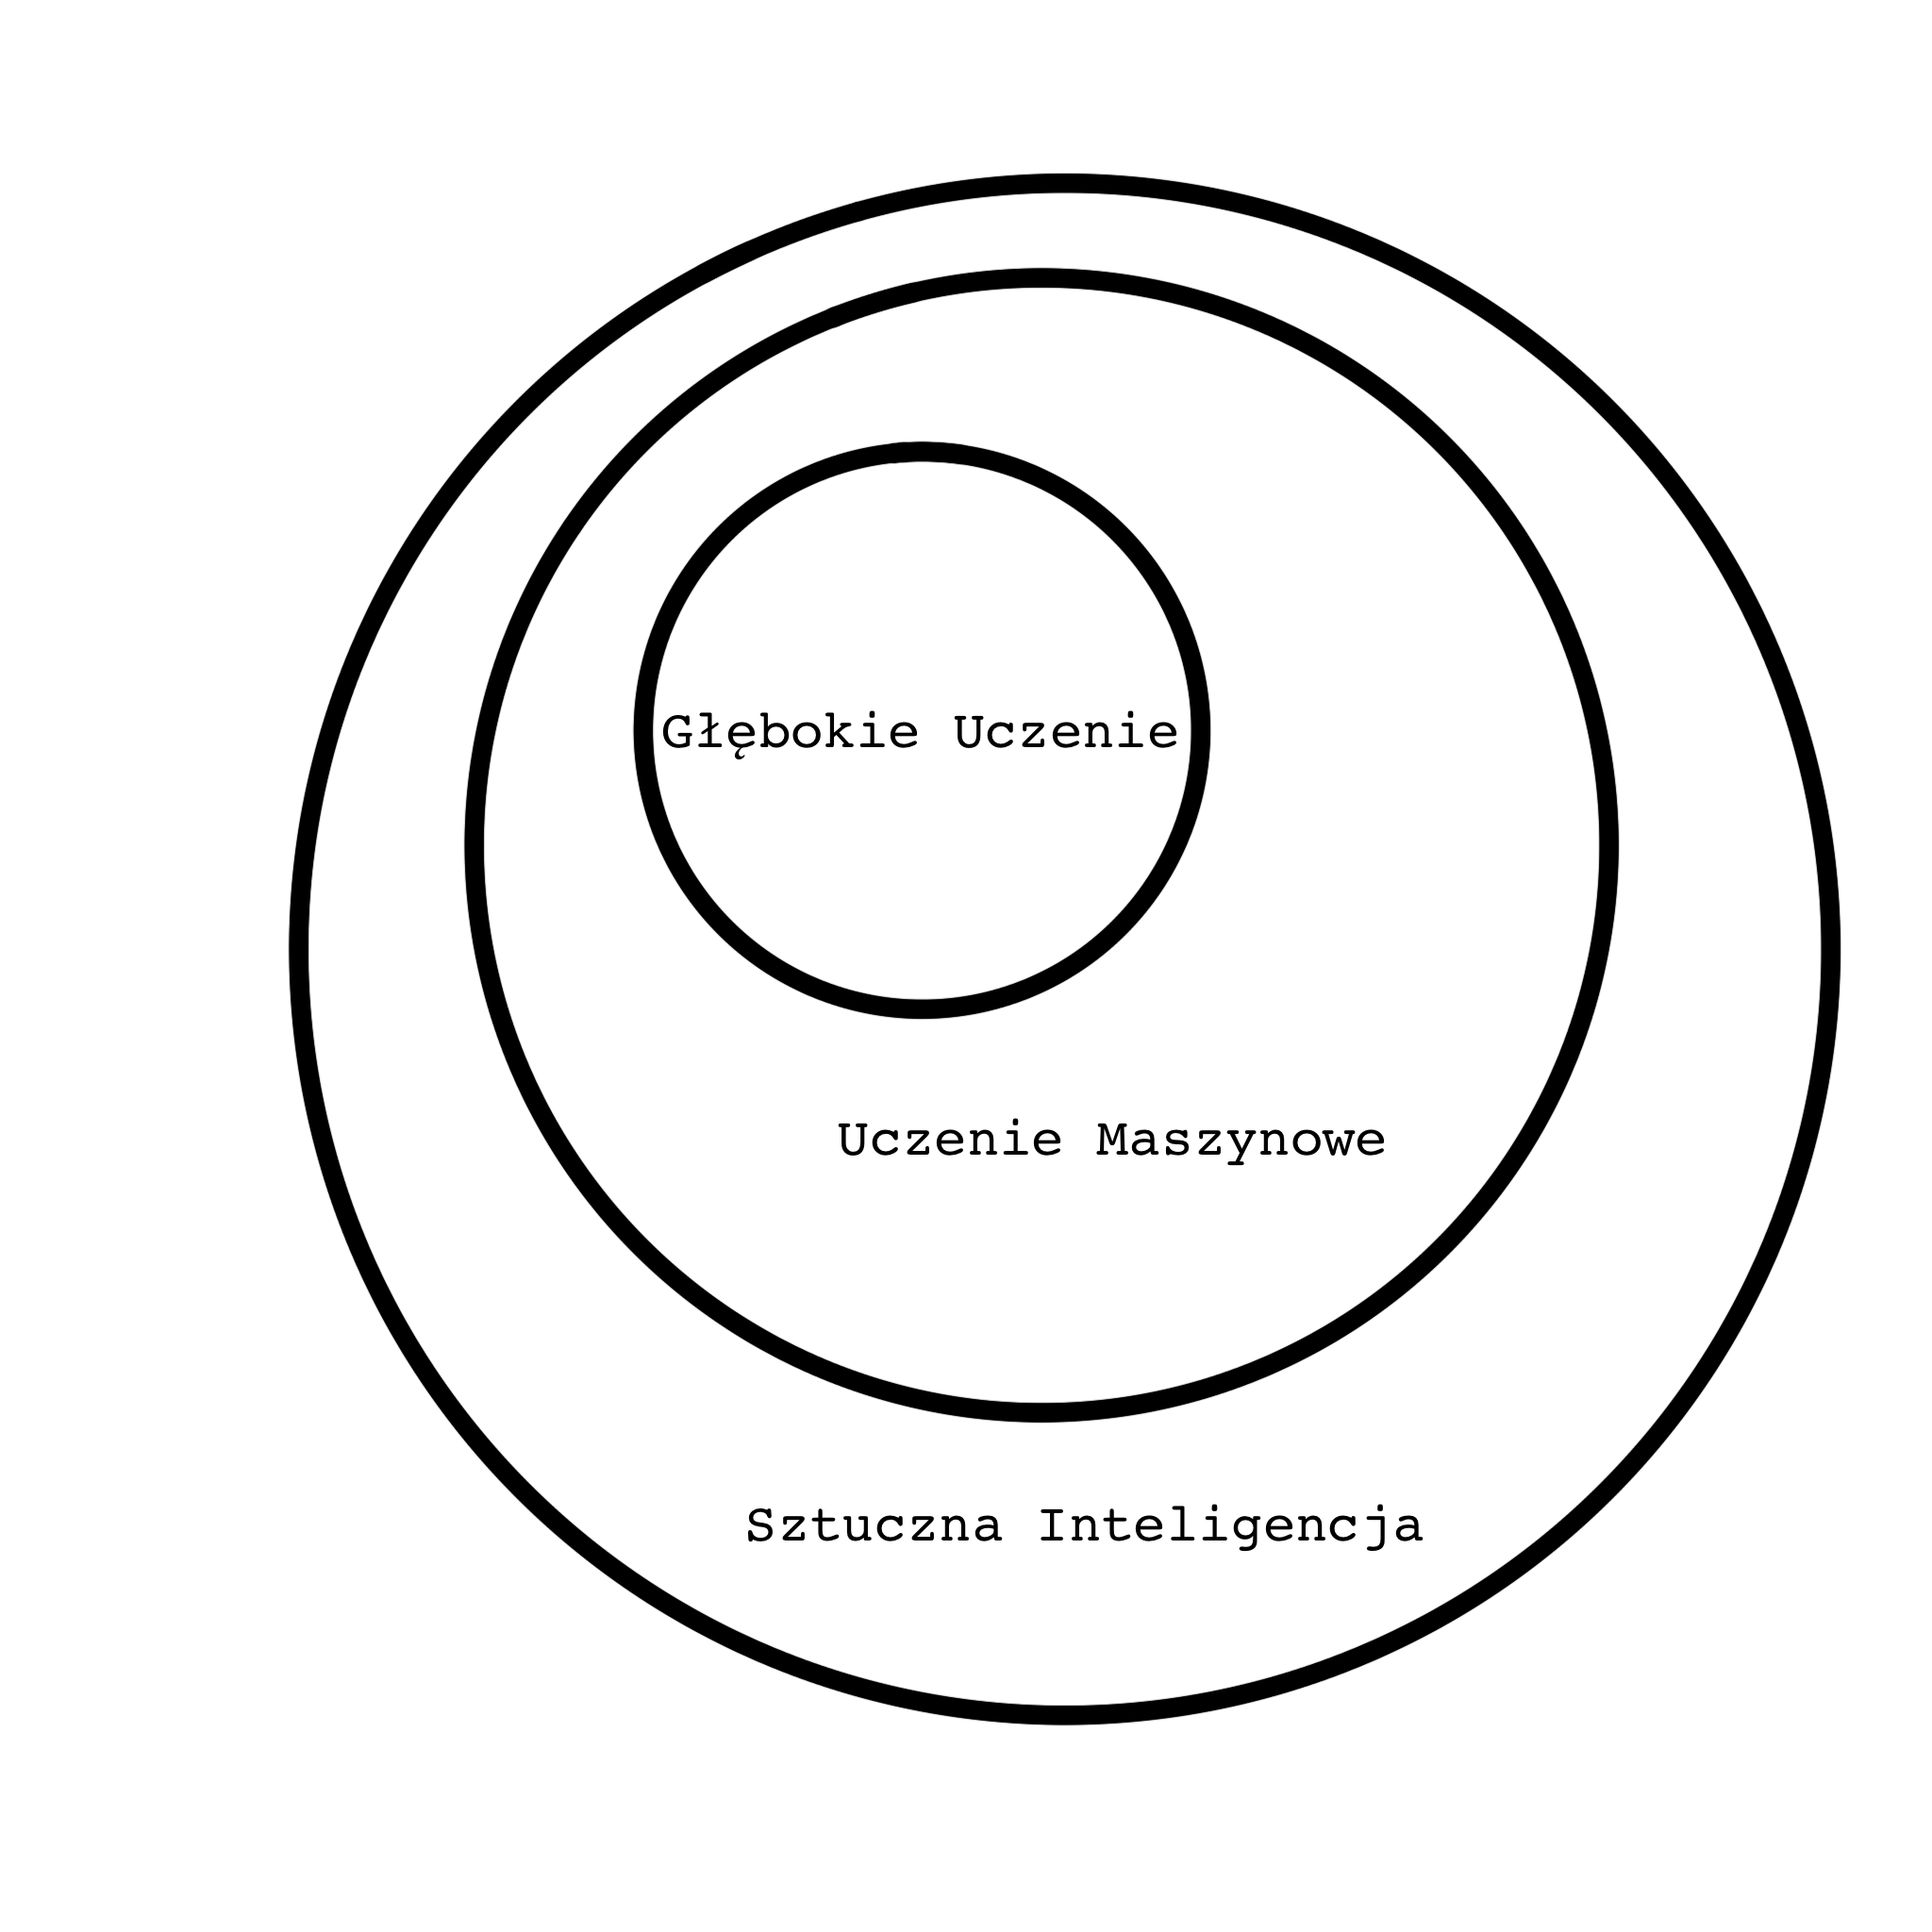
\includegraphics[width=.8\hsize]{fig/1}
\caption{Schemat zależności pomiędzy głębokim uczeniem, uczeniem maszynowym a sztuczną integencją\label{RYS.1}}
\source{Opracowanie własne}
\end{figure}


	


\chapter{Widzenie komputerowe  }

Możliwośc interpretacji i przetwarzania obrazu przez programy zostało zrewolucjonizowane
przez wprowadzenie konwolucyjnych sieci neuronowych, a aplikacje oparte na analizie obrazu zyskały nowy wymiar możliwości. 

W tym rozdziale zostaną omówione podstawowe definicje związane, a następnie przedstawiony zostanie przykład obrazujący, według jakiego wzorca konstruowane są sieci neuronowe. Omówione zostanie również 
możliwości odczytu, przetwarzania oraz zapisu obrazów.

\section{Neuron  \label{s:dsssl}}

Neuronem określamy najbardziej elementarną cząstkę modelu uczenia maszynowego, który jest jest podstawowym budulcem sieci neuronowej. Często jest on pojedynczą liczbą np. odcień szarości (\textit{ang. Grayscale Value}) dla pojedynczego piksela w przypadku czarno-białego obrazka. Połączenia miedzy neuronami obrazowane się za pomocą grafu (Rysunek 2.1).

\section{Sieci Neuronowe   \label{s:dsssl}}

Sieci Neuronowe (\textit{ang. Neural Networks}) to teoretyczny paradygmat struktur matematycznych inspirowany układem synaps i połączeń między nimi w mózgu. Składowymi sieci neuronowych są neurony oraz połączenia między nimi. Sieci neuronowe otrzymują liczbowe dane wejściowe i przekazują liczbowe dane wyjściowe. Może to być np. klasyfikacja, tłumaczenie lub obliczenie. Sieci neuronowe dzieli się na warstwy (ang. Layers), w których każda przetwarzana jest z uwzglądnieniem poprzedniej [7, 8].



\section{Przykład  \label{s:dsssl}}

Posłużmy się przykładem prostej sieci neuronowej, która ma za zadanie rozpoznać pisane cyfry. Jest to najbardziej elementarny przykład w dziedzinie uczenia maszynowego.
W przypadku analizy obrazka 64x64 piksele jedna warstwa sieci neuronowej składać będzie się z 4096 neuronów, czyli łącznej liczby pikseli w macierzy. Odniesienia do tego przykładu znajdą się w dalszych podrodziałach.

\begin{figure}[!tbh]
\centering
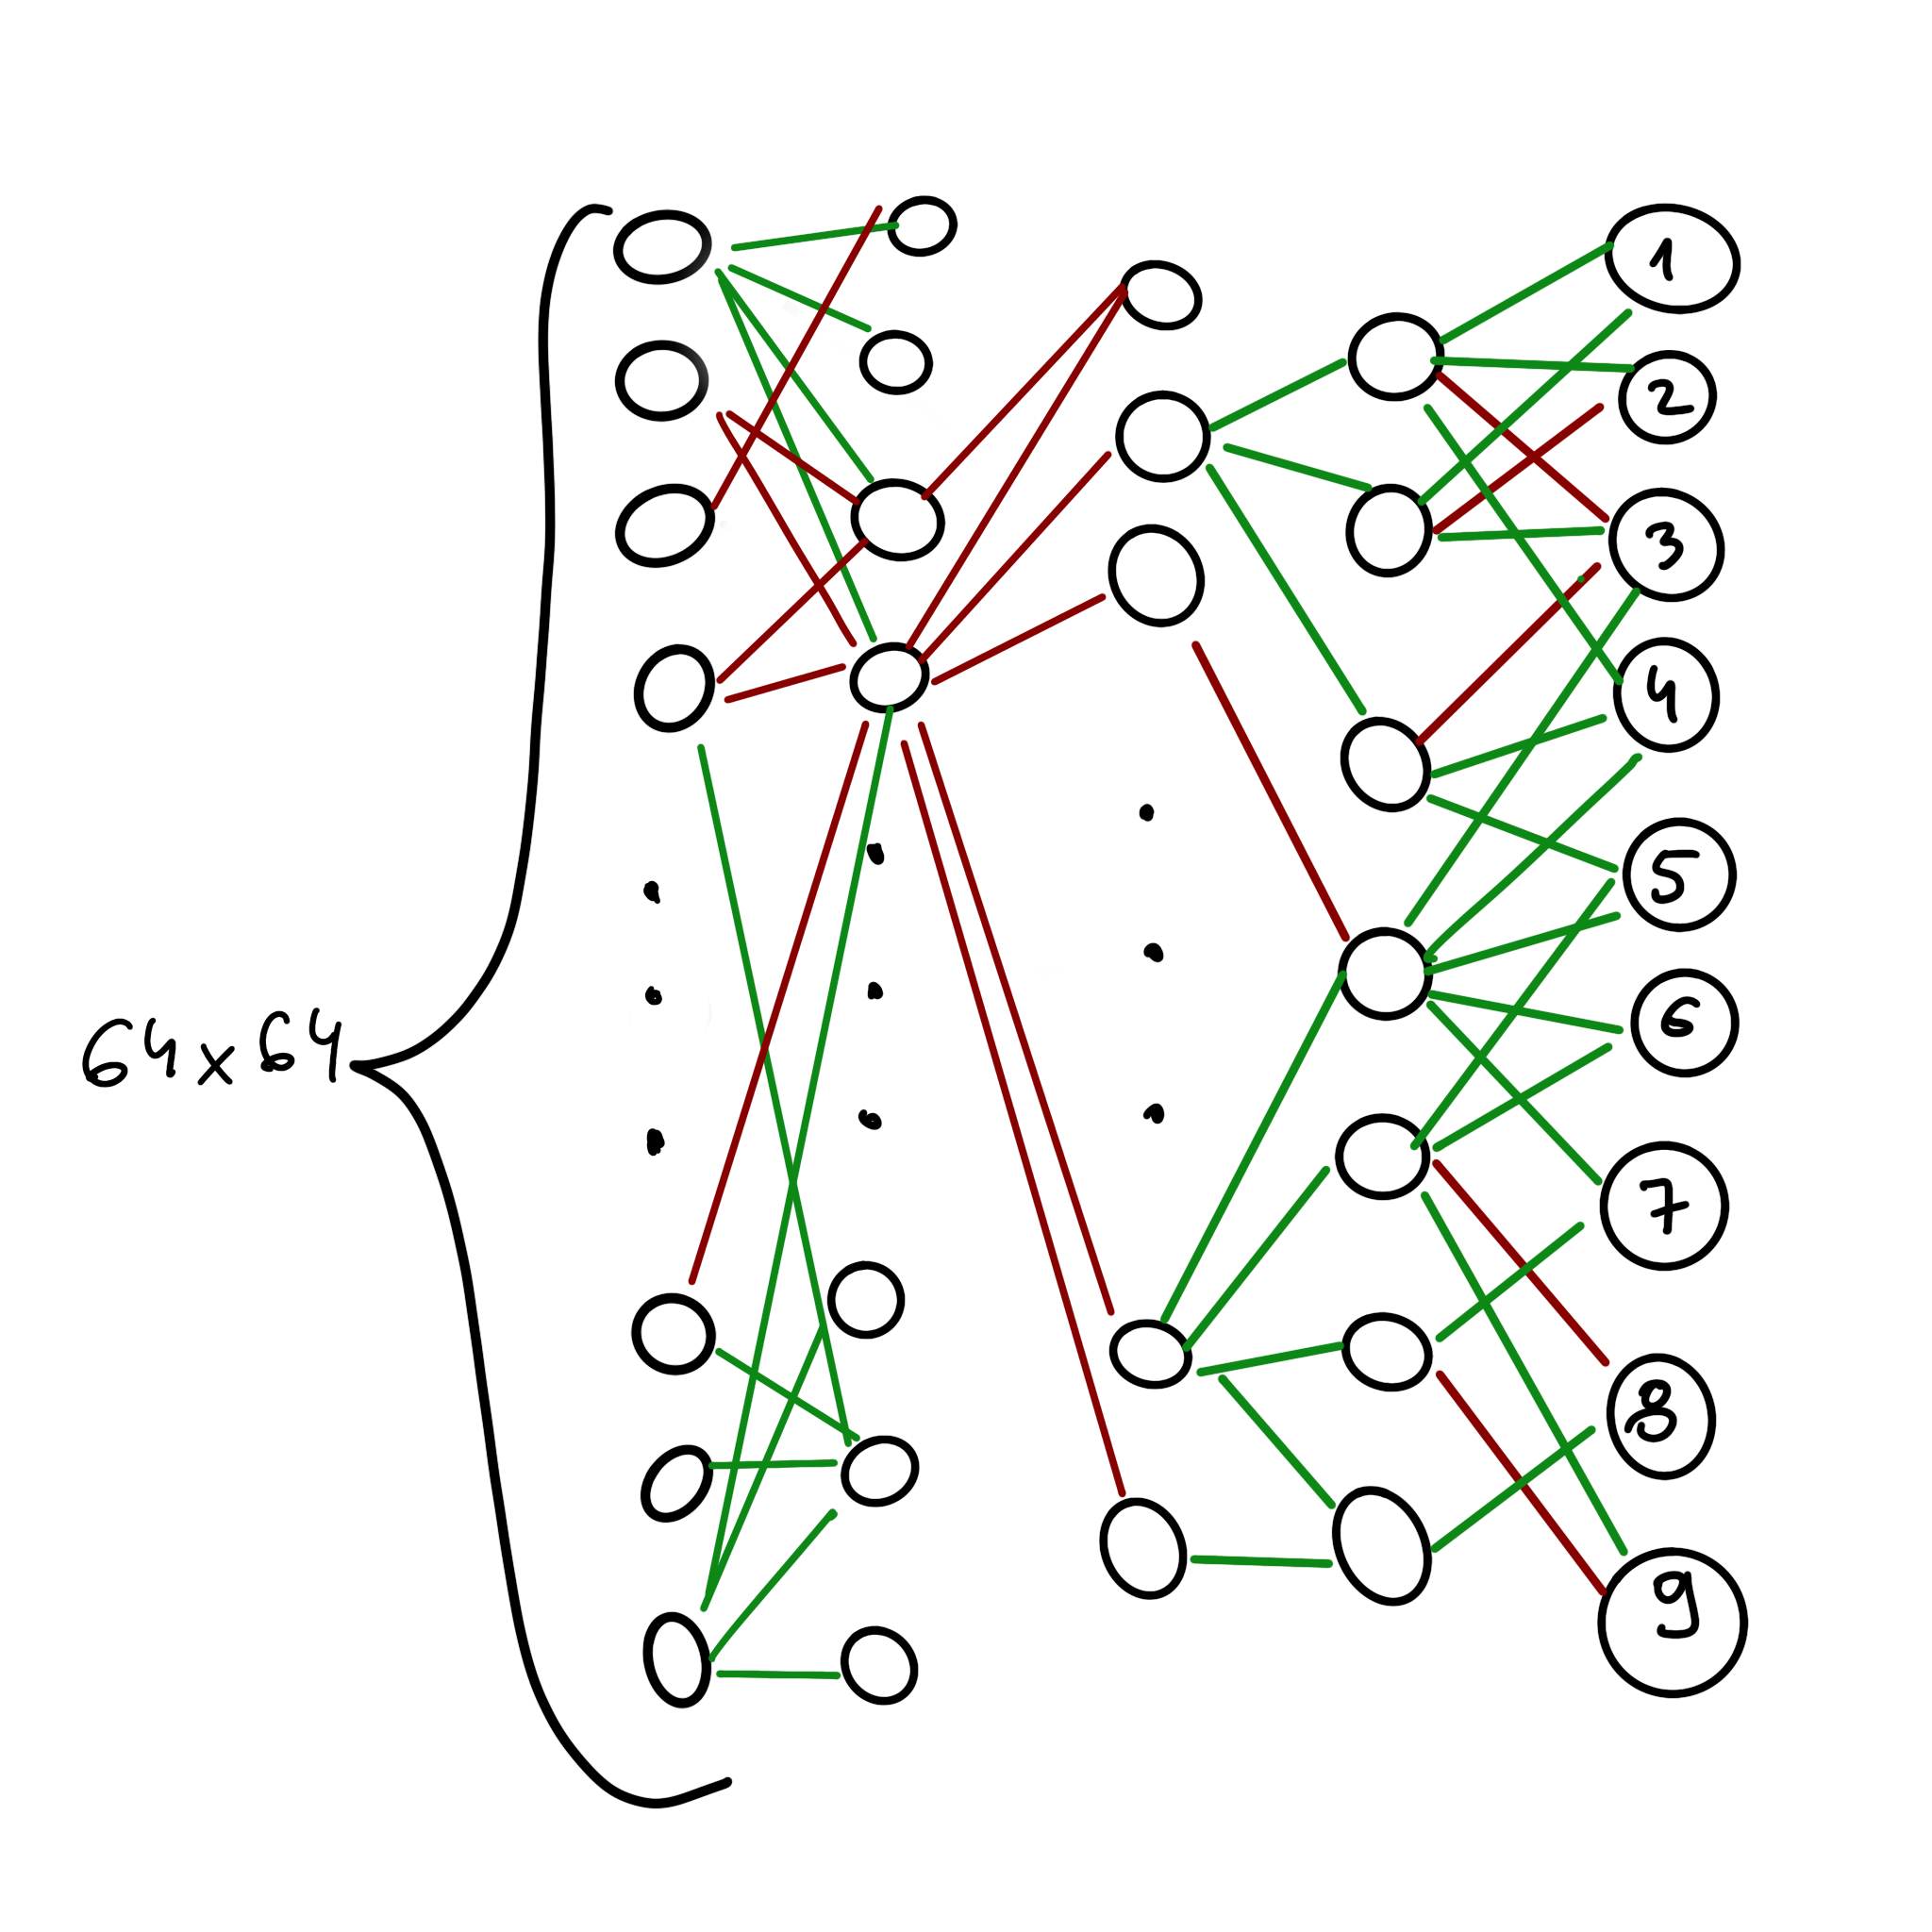
\includegraphics[width=.8\hsize]{fig/2}
\caption{Układ neuronow dla obrazka 64x64 px\label{RYS.2}}
\source{Opracowanie własne}
\end{figure}


\section{Konwolucyjne Sieci Neuronowe  \label{s:dsssl}}


Konwolucyjne Sieci Neuronowe (\textit{ang. Convolutional Neural Network}) zwane też splotowymi to charakterystyczny dla głębokiego uczenia typ sieci neuronowych, w których część warstw w środku sieci jest ukryta (\textit{ang. Hidden Layers}).

Konwolucyjcyjne Sieci Neuronowe działają na zasadzie ekstrakcji cech (\textit{ang. Feature Extraction}) na zbiorach danych. Zbudowane są z sekwencyjnych warstw, gdzie każda warstwa dokonuje ekstrakcji cech coraz to wyższego poziomu.





\begin{figure}[!tbh]
\centering
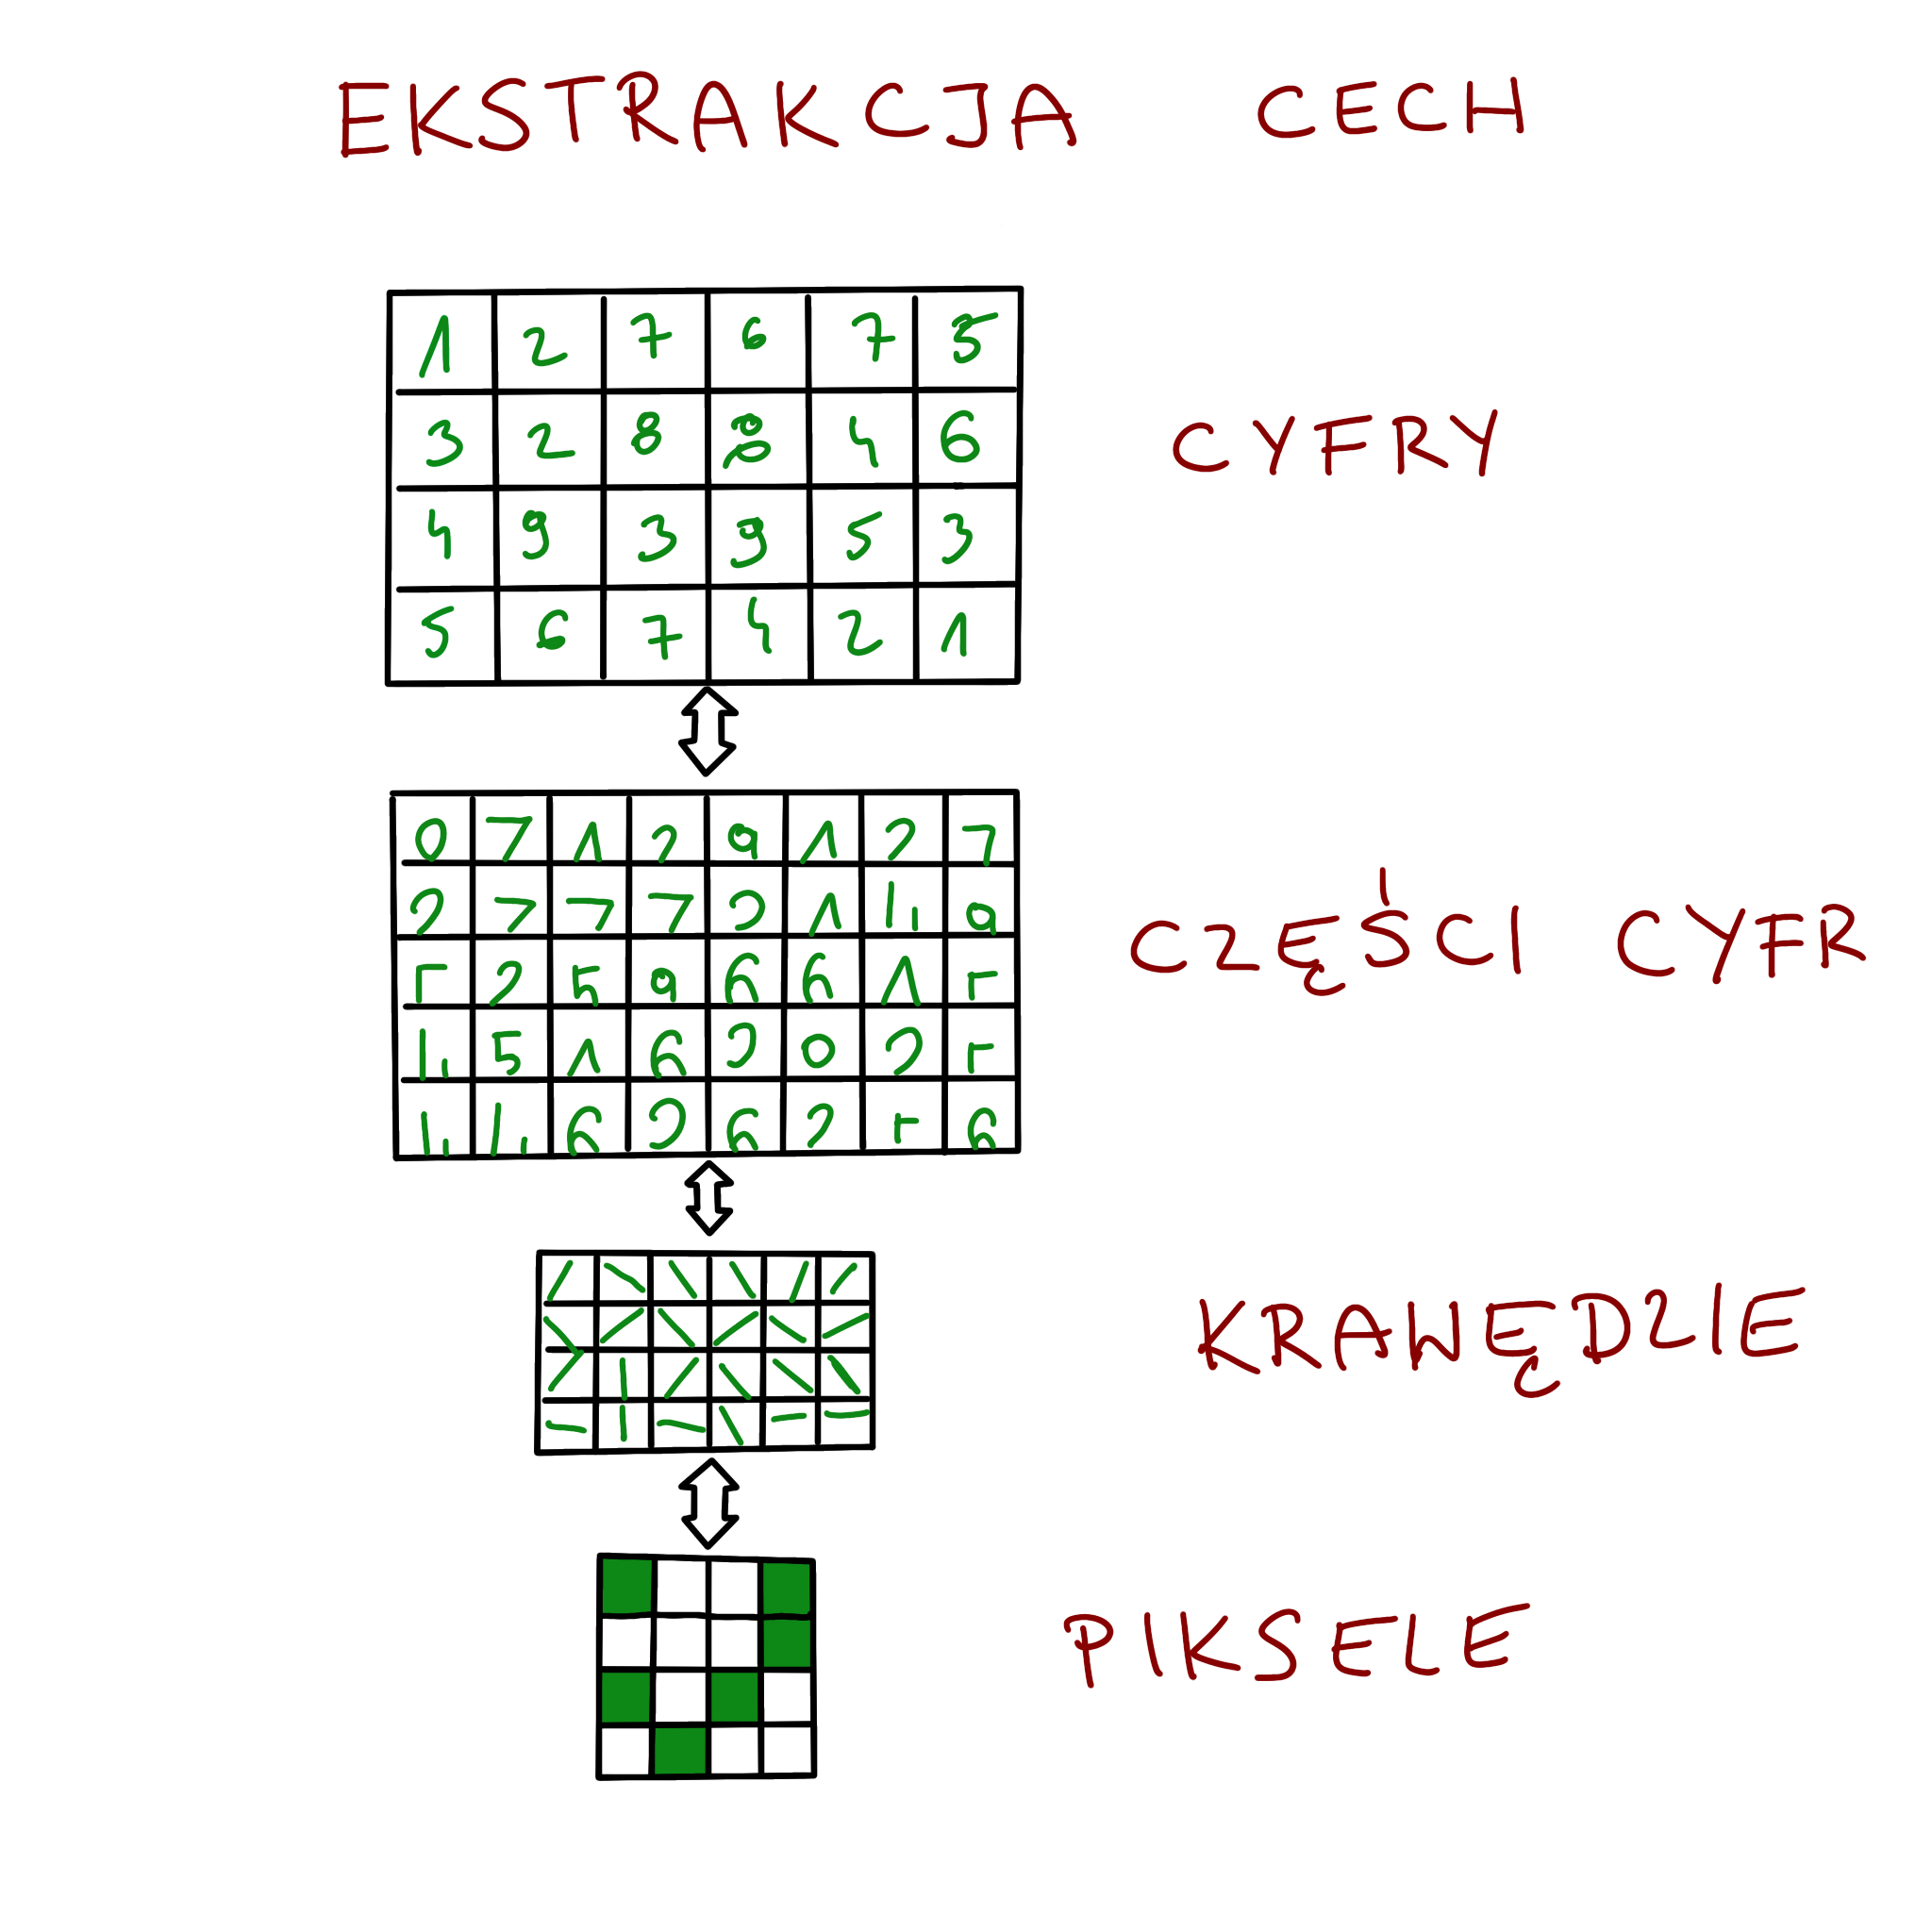
\includegraphics[width=.8\hsize]{fig/10}
\caption{Przykład ekstrakcji cech w konwolucyjnej sieci neuronowej\label{RYS.2}}
\source{Opracowanie własne}
\end{figure}

Sieci konwolucyjne poprzez trening są w stanie nauczyć się, jakie cechy szczególne obrazu pomagają w jego klasyfikacji. Jest to możliwe dzięki zastosowaniu filtrów badających relacje pikselli będących w sąsiedztwie. Warto jednak wspomnieć o innych sieciach np. "Long short-term memory network", która swoje zastosowanie ma w analizie dźwięku. Konwolucyjna sieć neuronowa składa się z jednej lub wielu warstw klastrów połączeń.

 Sprawdzają się one przy analizie obrazów.  Mogą być one automatycznie dostosowywane, aby specjalizować się w danym problemie.

Dane są często dzielone na osobne zestawy próbek szkoleniowych i próbek walidacyjnych, co pozwala na ocenę modelu na podstawie danych, na których nie był szkolony.





\section{Funkcja Aktywacji  \label{s:dsssl}}

Funkcja aktywacji  (\textit{ang. Activation Function}) ma na celu skoncentrowanie wyników poprzedniej operacji liniowej w danym zakresie.
Aktywacja z poprzedniej warstwy, determinuje aktywację w kolejnych aż do samego końca. 

Wartość każdego neuronu w sieci to funkcja, która przyjmuje dane wejściowe ze wszystkich neuronów z poprzedniej warstwy i przetwarza to na wartość od 0 do 1, 0 to czarny, a 1 to biały. Wartości te zwana są “aktywacją” lub “funkcją aktywacji”.


\begin{figure}[!tbh]
\centering
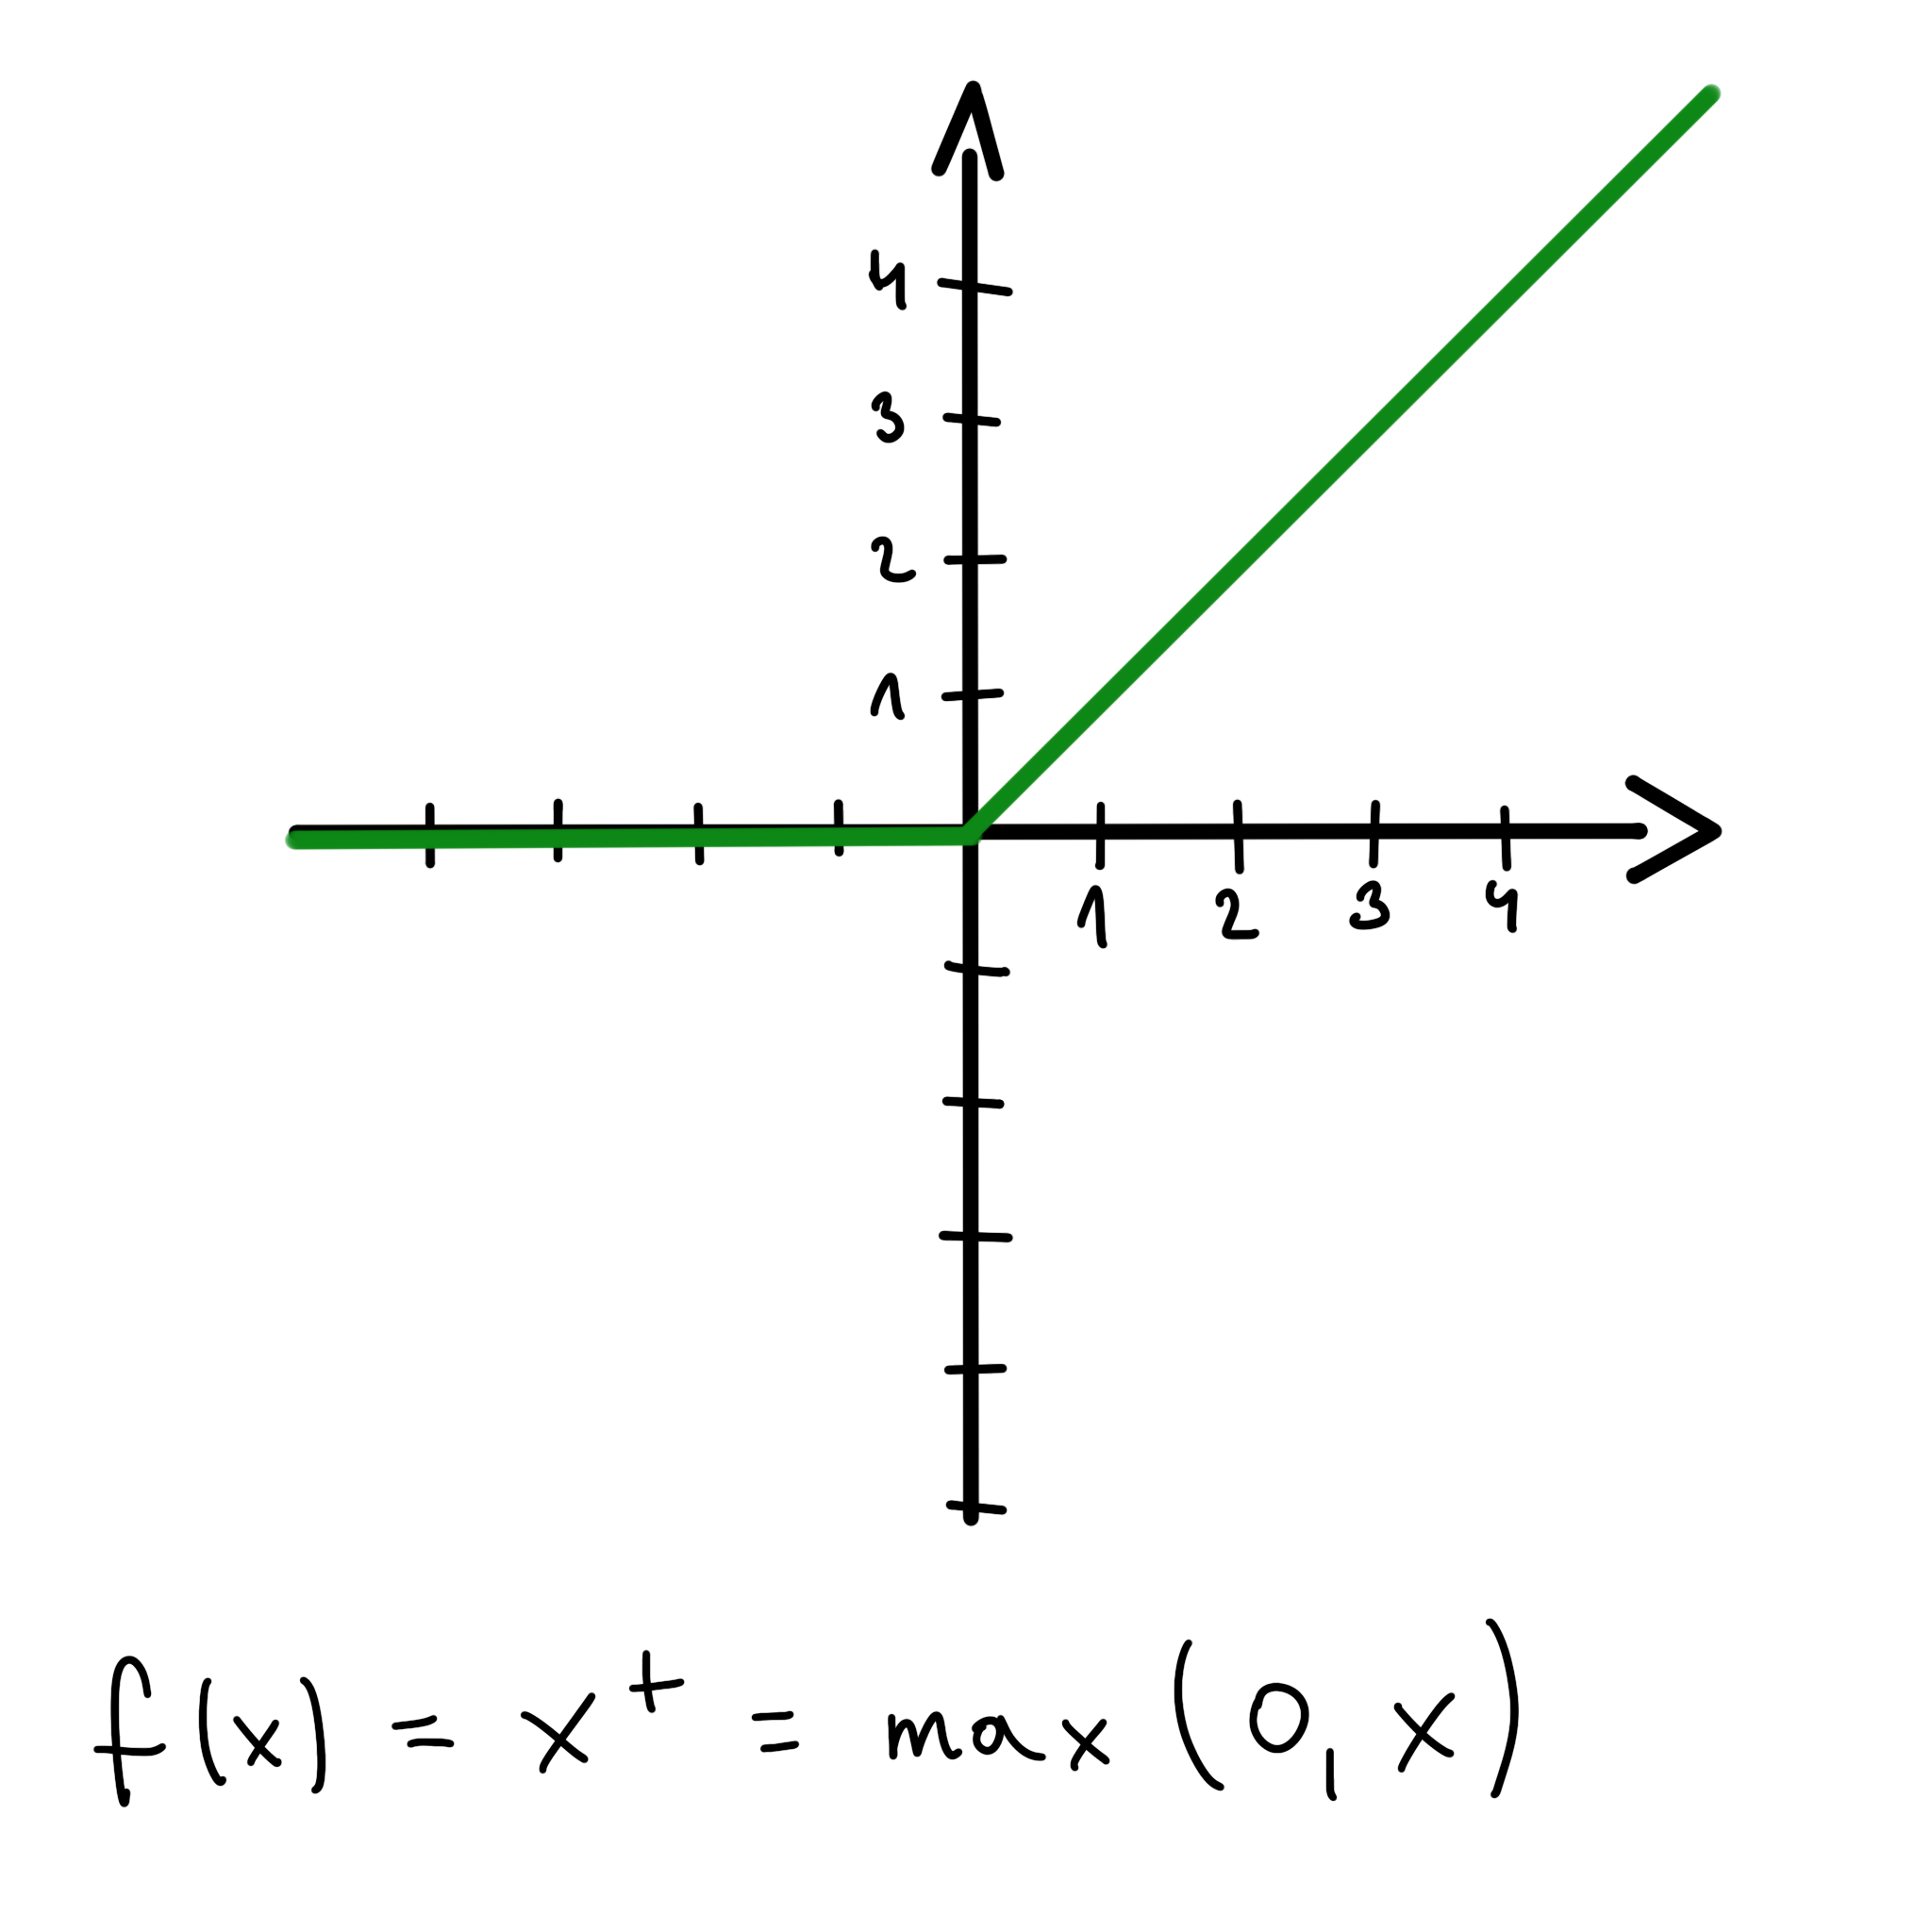
\includegraphics[width=.8\hsize]{fig/4}
\caption{Funkcja ReLU: $f(x) = max(0, x)$\label{RYS.3}}
\source{Opracowanie własne}
\end{figure}

Dla każdego neuronu wykonywana jest operacja matematyczna:

\begin{equation}
neuron  = φ (w * x + b)
\end{equation}

\begin{itemize}
\item “x” jest wkładem do obliczeń pojedynczego neuronu, w przypadku rozpoznawania cyfr x jest wartością od 0 do 1, czyli odcieniem szarości dla danego piksela
\item “w” jest wagą, jest to wartość, która na swój sposób określa jak istotny jest wynik danych neuronów. W przypadku rozpoznawania cyfr pisanych odręcznie, piksele na skraju obrazka będą miały mniejsze znaczenie niż te w okolicach jego centrum. Wagi mówią, jaki wzór pikselowy odbiera neuron w kolejnej warstwie.
\item "b" to odchylenie (bias), który mówi, jak wysoka musi być suma ważona, zanim neuron zacznie być znacząco aktywny.
\end{itemize}

\begin{figure}[!tbh]
\centering
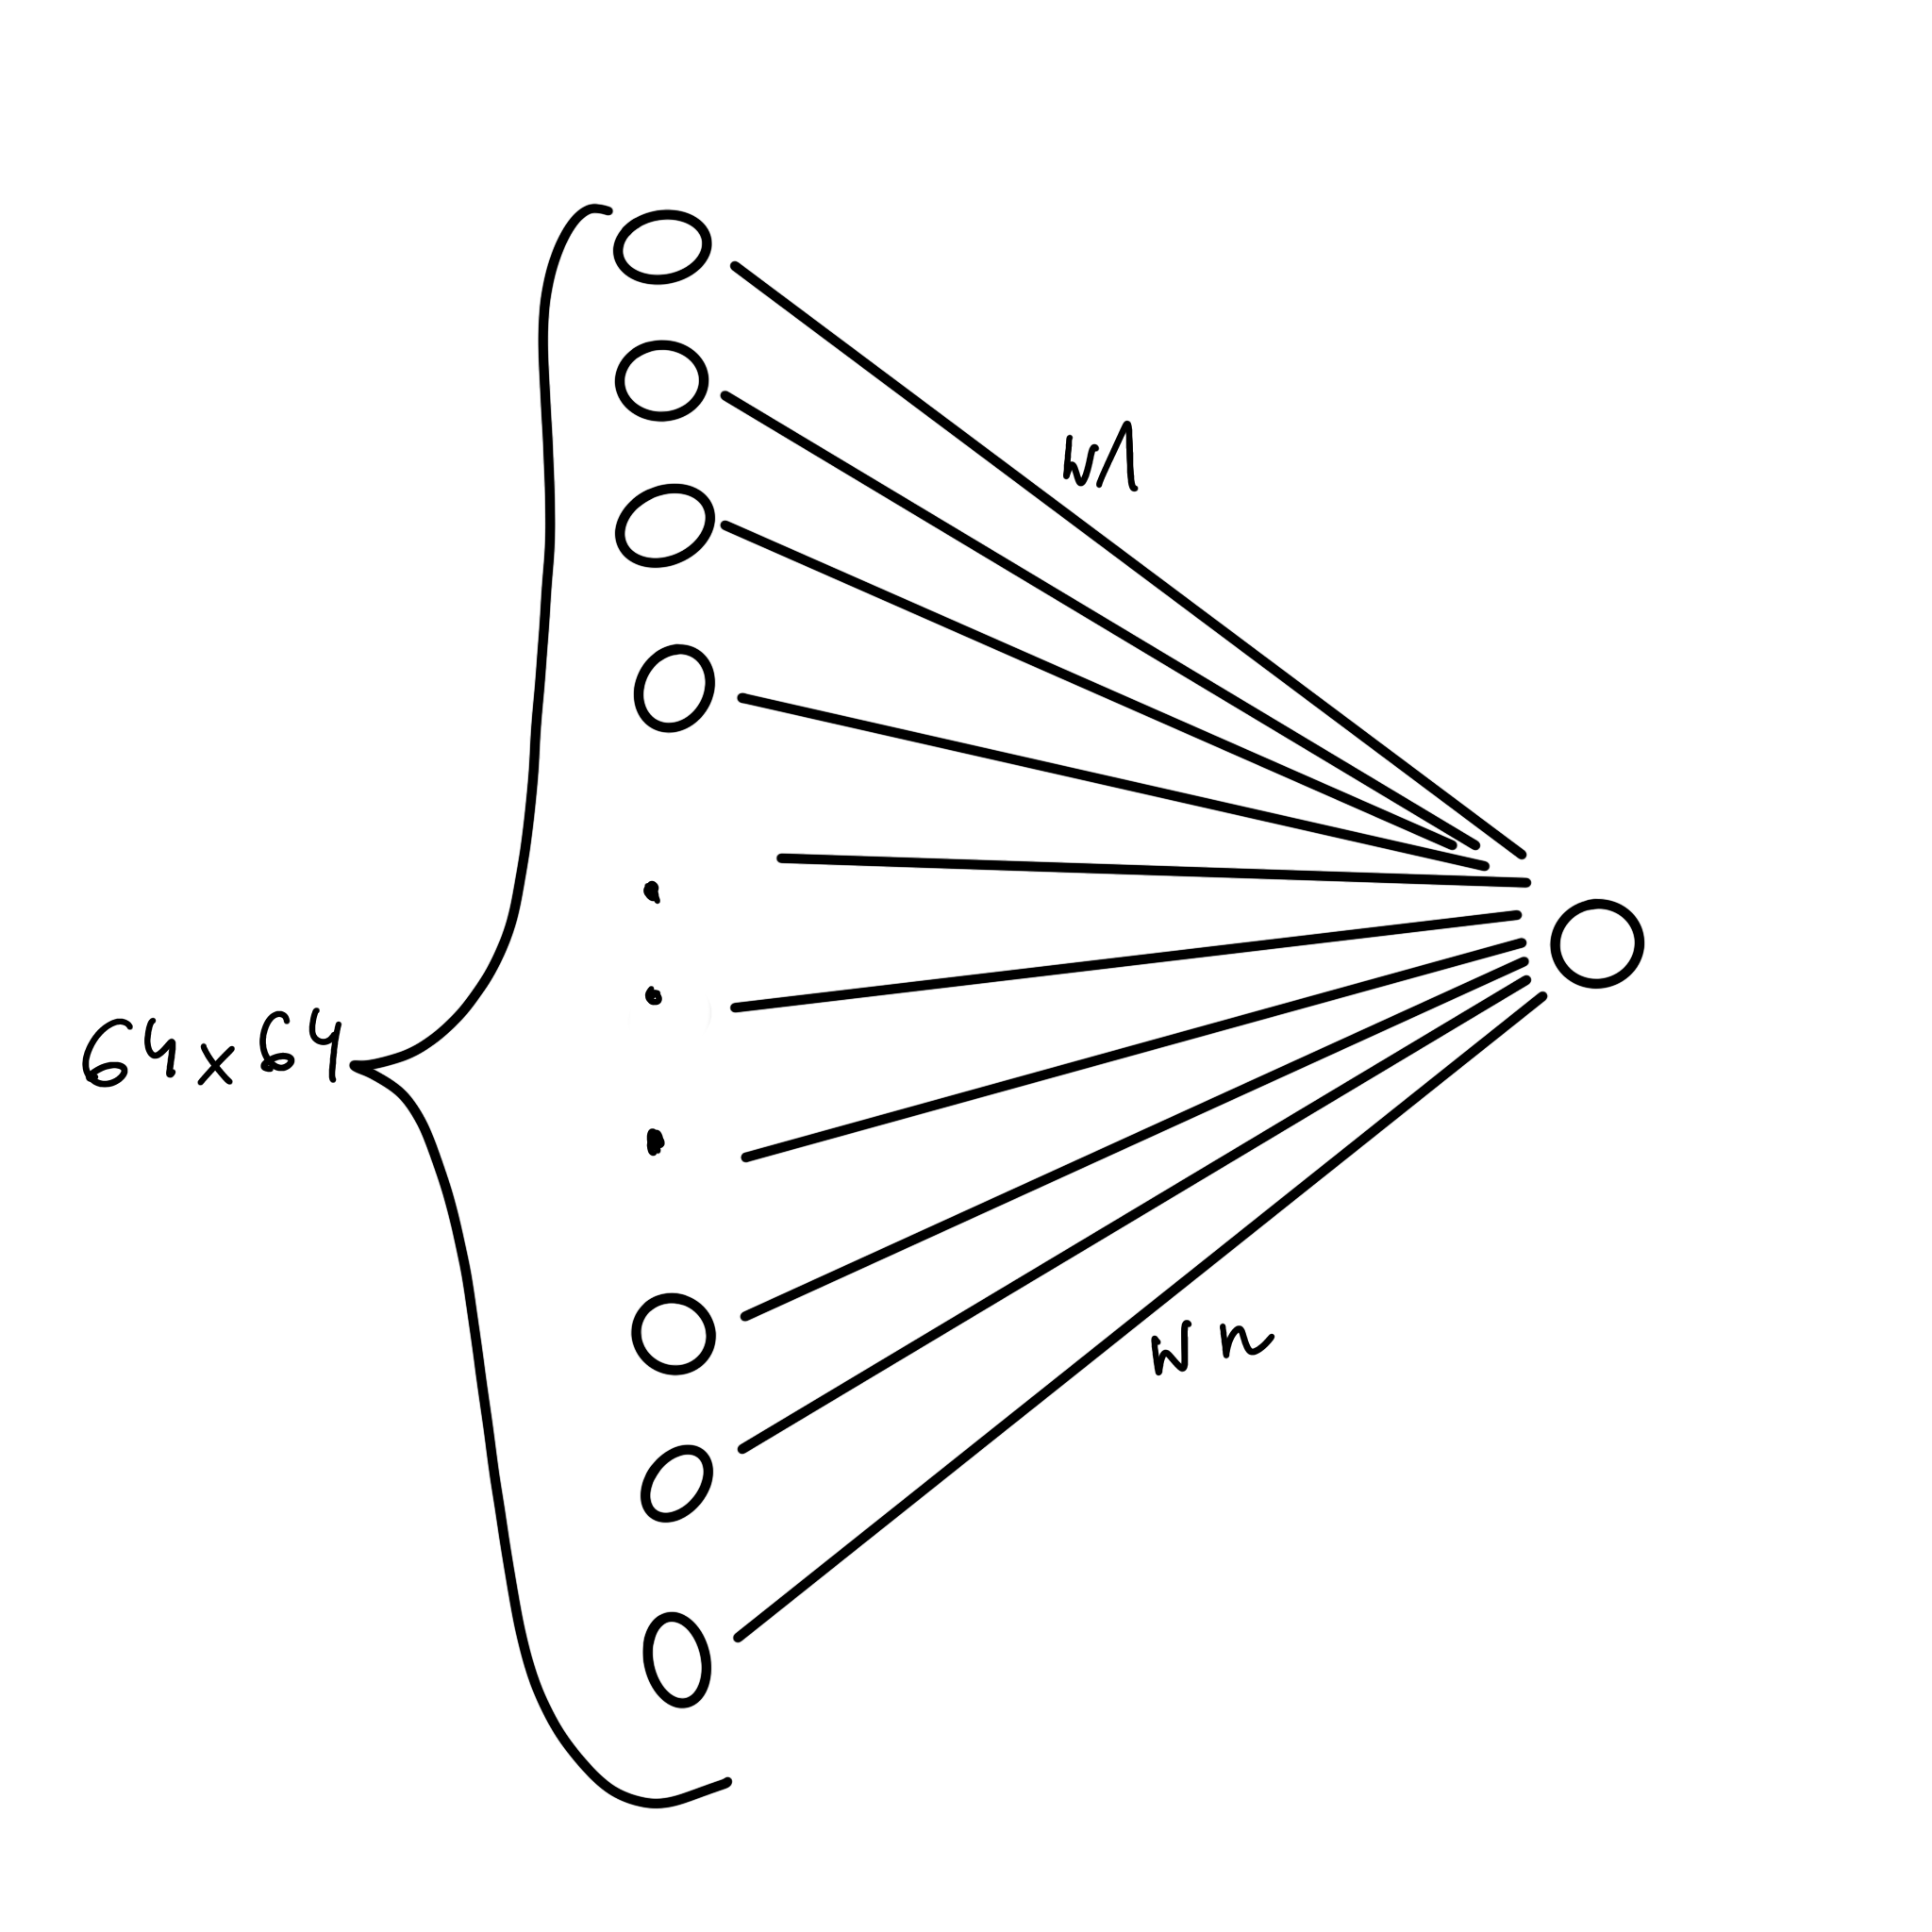
\includegraphics[width=.8\hsize]{fig/3}
\caption{Przypisywanie wag dla poszczegónych neuronów\label{RYS.3}}
\source{Opracowanie własne}
\end{figure}

W każdej warstwie  wartość w neuronie po dodaniu odchylenia i przemnożeniu przez wagę w celu identyfikacji tylko “ważnych” wartości całość przeliczamy jeszcze przez funkcję aktywacyjną. 
Tak zwana warstwa ReLU usuwa ujemne wartości z mapy aktywacji, ustawiając je na zero, co zwiększa nieliniowe właściwości funkcji decyzyjnej i całej sieci.


 Wagi mnożymy z aktywacją, aby pomagały w określeniu stopnia aktywacji, zachowujemy je w przedziale od 0 do 1.
 
 W przykładowej sieci rozpoznawającej liczby pisane ostatnią warstwą jest 10 neuronów z wartościami cyfr od 0 do 10 i ta z największą wartością aktywacji zostaje wybrana. 
 
 \section{Funkcja Strat \label{s:dsssl}}
 
Funkcja strat (\textit{ang. Loss Function}) to miara błędu w wykonywaniu zadania, takiego jak błąd między przewidywanymi wyjściami a mierzonymi wartościami. Celem jest, aby wartość funkcja strat była jak najniższa. 
Funkcja strat jest sumą kwadratów różnicy, między ostatnimi neuronami w sieci, a podanym przez użytkownika wynikiem. Średnią stratę dla całej sieci (\textit{ang. Mean Squared Error}) wyliczamy ze wzoru:  

$$MSE=\frac{\sum_{i=1}^{n} (y_i - y_i)}{n}$$

gdzie: 

\begin{itemize}
\item $n$ jest liczbą neuronów w sieci
\item $y_i$ jest wartością neuronu o indeksie $i$ 
\item $y_i'$ jest spodziewaną warością neuronu o indeksie $i$ 
\end{itemize}

Wyznacznikiem uczenia sieci neuronowej jest zmniejszanie funcji strat. 


 \section{Metoda Gradientu Prostego\label{s:dsssl}}

Metoda Gradientu Prostego (\textit{ang. Gradient descent}) to opracowany przez Cauchy'ego w 1847 r. [6] iteracyjny algorytm optymalizacji pierwszego rzędu do znajdowania lokalnego minimum funkcji różniczkowalnej.

W dziedzinie uczenia maszynowego Metoda Gradientu Prostego jest użyteczna przy estymacji parametrów funkcji. 


\begin{figure}[!tbh]
\centering
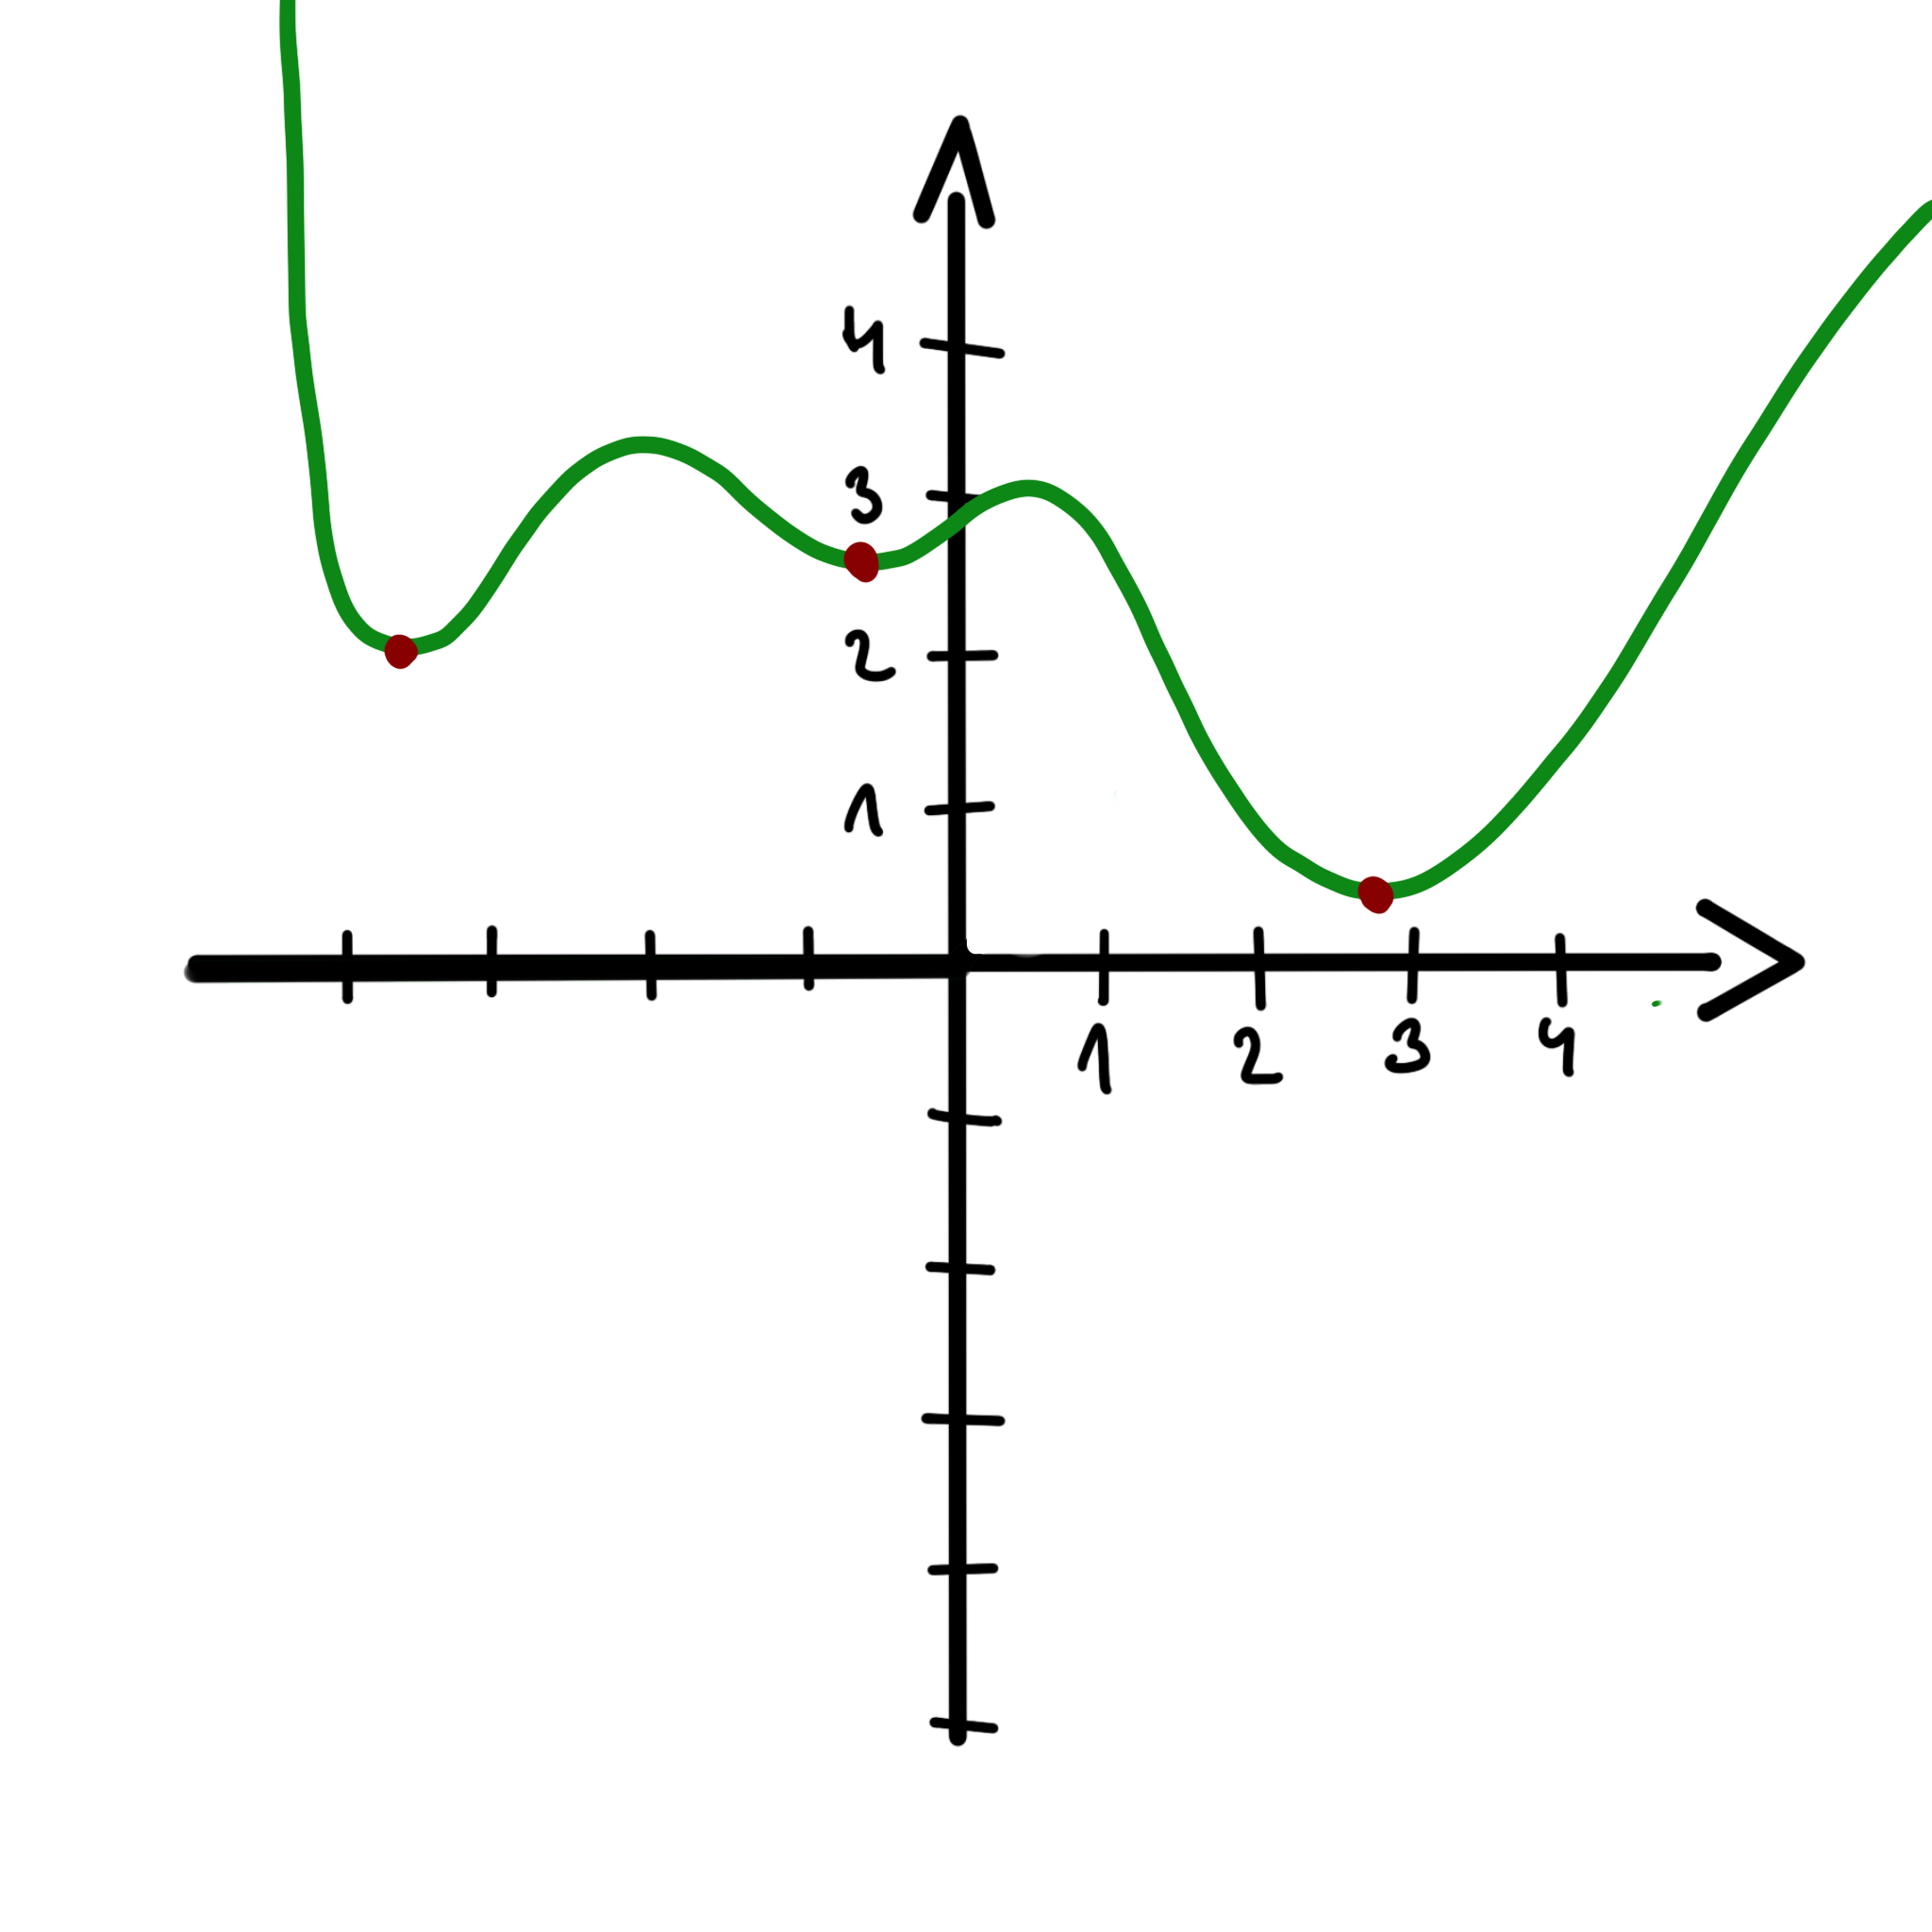
\includegraphics[width=.8\hsize]{fig/11}
\caption{Minima lokalne w funckji, znalezione metodą gradientu prostego\label{RYS.3}}
\source{Opracowanie własne}
\end{figure}

Aby znaleźć lokalne minimum funkcji za pomocą opadania gradientu, wykonujemy kroki proporcjonalne do ujemnego gradientu (lub przybliżonego gradientu) funkcji w bieżącym punkcie.  [16]. 

Im więcej kroków optymalizacji tym bardziej efektowny będzie transfer stylu.
Przykład użycia takiego optymalizatora znajduje się w rozdziale 5.3.

\section{Propagacja Wsteczna\label{s:dsssl}}

W uczeniu maszynowym propagowanie wsteczne (\textit{ang. Backpropagation}) jest szeroko stosowanym algorytmem w uczeniu sieci neuronowych. Algorytm ten edytuje wagi oraz odchylenia każdego połączenia neuronu w sieci tak, aby minimalizowć funkcję strat.

Przy dopasowywaniu sieci neuronowej propagacja wsteczna oblicza metodą gradientu prostego funkcję strat w odniesieniu do wag w całej sieci. Dzięki wydajności metody gradientu prostego możliwe jest szkolenie sieci wielowarstwowych.

Algorytm wstecznej propagacji działa poprzez obliczenie gradientu funkcji strat w odniesieniu do każdej wagi według reguły łańcuchowej, obliczanie gradientu pojedynczej warstwy na raz, iterowanie wstecz od ostatniej warstwy. 


 \section{RGB\label{s:dsssl}}
 
 W przypadku algorytmu rozpoznjającego cyfry, obraz interpretowany przez komputer był w postaci dwuwymiarowej macierzy, z wartościami od 0 do 1. W przypadku algorytmów do innych zastosowań takich jak rozpoznawanie gatunków kwiatów lub znaków drogowych może okazać to się za mało. Analiza obrazów kolorowych zwiększa złożonośc sieci neuronowych. 
 
Istnieje kilka sposobów kodowania kolorów na liczby. Najpopularniejszym jest
RGB (\textit{ang. Red, Green, Blue}), który określa kolor za pomocą trzech liczb reprezentujących intensywność czerwieni, zieleni i niebieskiego. 

W tym momencie kolorowy obrazek jest obiektem podobnym do tablicy o trzech wymiarach: dwóch wymiarach przestrzennych (szerokość i wysokość) i trzecim wymiarze odpowiadającym kanałom czerwonym, zielonym i niebieskim. 

Każdy kolor będzie reprezentowany jako 8-bitowa liczba całkowita, jak w większości formatów fotograficznych ze standardowych aparatów konsumenckich. [2]

Wczytany obraz (np. w formacie *.jpg) należy przekrztałcić w wielowymiarową tablicę, która układa obraz w sposób zgodny z oczekiwaniami danego interfejsu programowania aplikacji, czyli API (\textit{ang. Application Programming Interface}) uczenia maszynowego.

\section{Tensor\label{s:dsssl}}


Tensor to struktura danych [4] przechowująca zbiór liczb, które są dostępne indywidualnie za pomocą indeksu i które mogą być indeksowane za pomocą wielu indeksów.

Termin tensor jest odnosi się do pojęcia przestrzeni, układów odniesienia i transformacji między nimi, oraz do uogólnienia wektorów i macierzy do dowolnej liczby wymiarów, jak pokazano na rysunku 2.6.
Tensory reprezentujące wartości w poszczególnych pikselach są często kodowane za pomocą liczb 8-bitowych, na przykład w kamerach konsumenckich. [2] W zastosowaniach medycznych, naukowych i przemysłowych nierzadko można znaleźć piksele o większej precyzji numerycznej, takie jak 12-bitowe i 16-bitowe.

 Ta precyzja zapewnia szerszy zakres lub zwiększoną czułość w przypadkach, w których piksel koduje informacje dotyczące właściwości fizycznej, takiej jak gęstość kości, temperatura lub głębokość.
 
 \begin{figure}[!tbh]
\centering
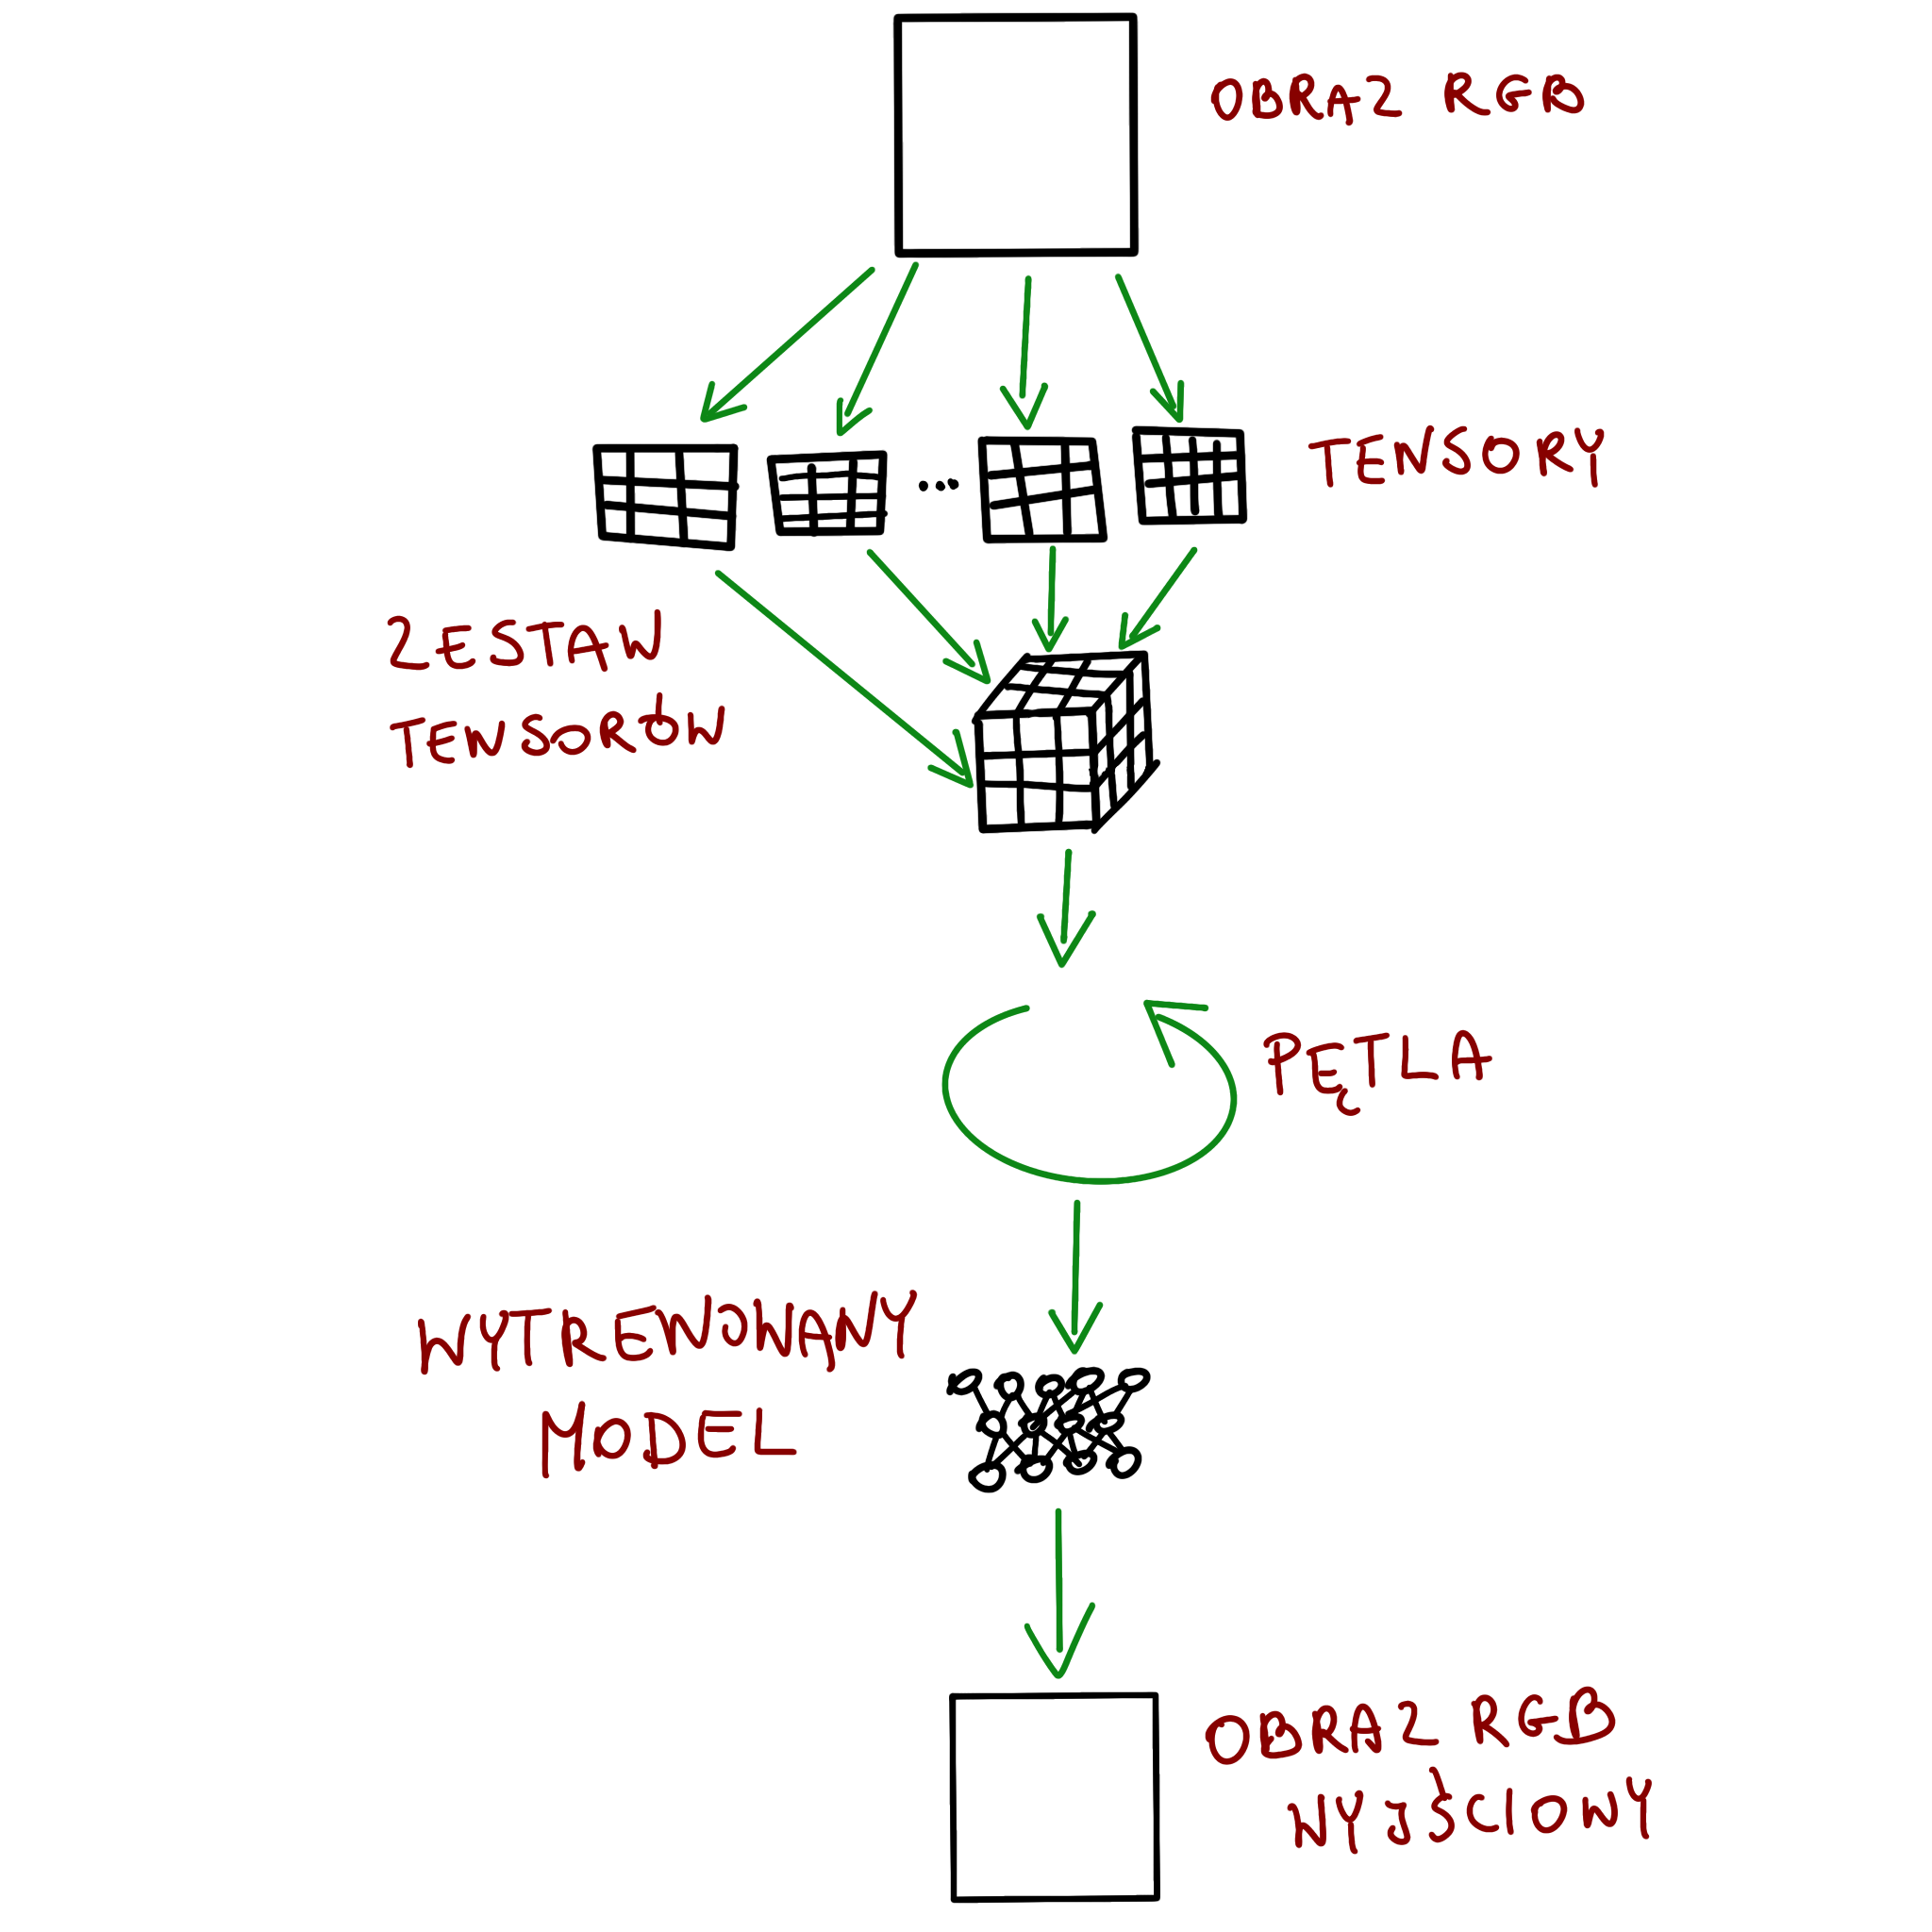
\includegraphics[width=.8\hsize]{fig/5}
\caption{Schemat przetwarzania obrazu\label{RYS.5}}
\source{Opracowanie własne}
\end{figure}

Sieci neuronowe pobierają tensory na wejściu i wytwarzają tensory na wyjściu. W rzeczywistości wszystkie operacje w sieci neuronowej i podczas optymalizacji są operacjami między tensorami, a wszystkie parametry (takie jak wagi i odchylenia) w sieci neuronowej również są tensorami.



Sieci neuronowe zwykle działają z wejściowymi tensorami zmiennoprzecinkowymi, wykazując najlepszą wydajność treningu, gdy dane wejściowe mieszczą się w przedziale od około 0 do 1 lub –1 do 1 (efekt definiowania ich bloków konstrukcyjnych). Sieci neuronowe wymagają przedstawiania danych jako wielowymiarowych tensorów numerycznych, często 32-bitowych liczb zmiennoprzecinkowych. [2]

Na rysunku 2.4 został przedstawiony schemat procesu operacji na obrazie.

Na tensorach można  wykonać kilka innych operacji na danych wejściowych, w tym przekształcenia geometryczne, takie jak obrót, skalowanie i kadrowanie. Operacje te mogą pomóc w szkoleniu lub mogą być wymagane, aby dowolne dane wejściowe były zgodne z wymaganiami wejściowymi sieci, takimi jak rozmiar obrazu.

 \section{Optymalizacja \label{s:dsssl}}
 
 Często w przypadku, gdy sieć neuronowa ma rozpoznawać zależności bazujące na kształtach (a rozpoznawanie cyfr pisanych właśnie takie jest) redukuje się dane wejściowe do minimum. Zamienia się wtedy kolorowy obrazek RGB na czarno-biały. Dzięki takiemu zabiegowi sieć neuronowa nie zawiera  niepotrzebnych danych takiech jak kolor i może to dać lepszą rozpoznawalność jak również wzrost wydajności zarówno w procesie szkolenia jak i działania klasyfikatora.  



 \section{Podsumowanie \label{s:dsssl}}
 
Podsumowując, można uważać za  poprawne stwierdzenie, iż uczenie sieci to tylko modyfikowanie wag oraz odchyleń tak, aby osiągać najlepsze rezultaty, czyli uczenie jest swego rodzaju szacowaniem parametrów.   



\chapter{Przegląd Wykorzystanych Narzędzi}

Przetwarzanie obrazu przy użyciu sieci neuronowych to interdyscyplinarne zagadnienie łączącę zagadnienia z matematyki, graficzki czy programowania. Przy tworzeniu implementacji tych zagadnień można sięgnąć po wiele dostępnych narzędzi. W tym rozdziale opisane zostaną natomiast te, użyte w implementacji Transferu Stylu opisanego szczegółowo wraz z przykładowym kodem w rozdziale 5.

\section{Python\label{s:dsssl}}

Język Python powstał już w latach dziewięćdziesiątych, a między innymi dzięki rewolucji uczenia maszynowego przeżywa swoją drugą młodość. Jest używany w przez największe platformy programistyczne (\textit{ang. Frameworks}) do uczenia maszynowego takie jak Tensorflow czy PyTorch (opisany w rodziale 4.3).
Jest to język, z którego w większości składa się API Blendera, czyli udostępniony dla programistów sposób do rozbudowywania tej aplikacji. Każda wersja Blendera ma wbudowaną już własną wersję Pythona. Na potrzeby tej pracy cała implementacja Transferu Stylu została napisana w tym języku.

\section{Blender\label{s:dsssl}}

Blender jest darmowym i otwartym oprogramowaniem do modelowania i renderowania obrazów oraz animacji trójwymiarowych. Pozwala on na pisanie w języku Python skryptów, które poszerzają podstawowe funkcjonalności Blendera.

\section{Wtyczki\label{s:dsssl}}

Jedną z wielu zalet środowiska Blender jest jego otwartość. Większość kodu jest otwarta i konfigurowalna, ułatwia to tworzenie rozszerzeń (wtyczek).

Wtyczki w Blenderze mogą istnieć w postaci pojedynczych skryptów 

\begin{equation}
*.py
\end{equation}

lub zestawu skryptów pakowanych w 
\begin{equation}
*.zip
\end{equation}

.zip. Uruchamiany wtedy jest plik 

\begin{equation}
\_\_init\_\_.py
\end{equation}


Zarówno wtyczki do Blendera jak i same operacje przy użyciu PyTorch’a mogą być tworzone na dowolnym systemie operacyjnym. Te narzędzia znacznie ułatwiają pracę nad tego typu oprogramowaniem.
 Do tego programu na potrzeby tej pracy utworzone zostało rozszerzenie, implementujące Transfer Stylu. 

\begin{figure}[!tbh]
\centering
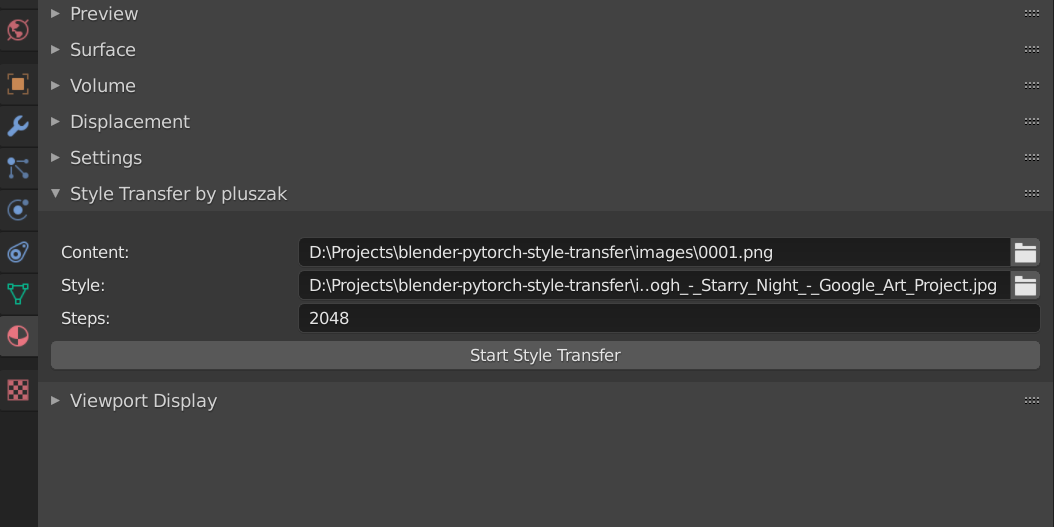
\includegraphics[width=.8\hsize]{fig/9}
\caption{Implementacja Transferu Stylu jako wtyczki w Blenderze\label{RYS.9}}
\source{Opracowanie własne}
\end{figure}

\section{PyCharm\label{s:dsssl}}
 PyCharm to zintegrowane środowisko programistyczne (\textit{ang. Integrated Development Environment IDE}) firmy JetBrains dla języka programowania Python. Zapewnia m.in.: edycję i analizę kodu źródłowego, graficzny debugger, uruchamianie testów jednostkowych, integrację z systemem kontroli wersji. 
 
 \section{Jupyter Notebook\label{s:dsssl}}
 
Jupyter Notebook to interaktywne środowisko pozwalające na wykonywanie kodu uczenia maszynowego po stronie serwera. Pozwala na szybkie debugowanie i testowanie kodu, między innymi biblioteki PyTorch.

 \section{CUDA\label{s:dsssl}}
 
CUDA (\textit{ang. Compute Unified Device Architecture}) jest to opracowana przez firmę Nvidia uniwersalna architektura procesorów wielordzeniowych (głównie kart graficznych) umożliwiająca wykorzystanie ich mocy obliczeniowej do rozwiązywania ogólnych problemów numerycznych w sposób wydajniejszy niż w tradycyjnych, sekwencyjnych procesorach ogólnego zastosowania. Charakteryzuje się ona wyższym współczynnikiem FLOPS (\textit{ang. Floating Point Operations Per Second}) czyli ilości operacji zmiennoprzecinkowych na sekundę.




\chapter{Przegląd Wykorzystanych Bibliotek}


Podobnie jak w przypdaku narzędzi jest wiele bibliotek w języku Python rozwiązujące te same zagdanienia. 
W tym rozdziale opisane zostaną natomiast te, użyte w implementacji Transferu Stylu opisanego szczegółowo wraz z przykładowym kodem w rozdziale 5.

 \section{PIP\label{s:dsssl}}
 PIP (\textit{ang. Pip Installs Python}) to standardowy system zarządzania rozszerzeniami i bibliotekami w Pythonie. Wszystkie inne zewnętrzne biblioteki Pythona instalowane są przy pomocy PIP.

\lstset{caption={Przykład instalacji PIP-a na danym Pythonie w systemie Windows}}
\begin{lstlisting}
python.exe -m ensurepip
\end{lstlisting}


 

    \section{PyTorch\label{s:dsssl}}
    
    
PyTorch to biblioteka, która ułatwia budowanie projektów głębokiego uczenia. [3] Pozwala wyrazić modele głębokiego uczenia w języku Python. Ta przystępność i łatwość użycia znalazły wczesnych użytkowników w społeczności badawczej, a od lat od wydania biblioteki stała się jednym z najważniejszych narzędzi do głębokiego uczenia dla szerokiego zakresu aplikacji.

Instalujemy ją przy pomocy wcześniej wspomnianego PIP-a:

\lstset{caption={Instalacja PyTorch przy użyciu  PIP-a}}
\begin{lstlisting}
python.exe -m pip install torch
\end{lstlisting}


Dzięki integracji bibliotek PyTorch ze standardową biblioteką Python i otaczającym ekosystemem, ładowanie najpopularniejszych rodzajów danych i konwertowanie ich do tensorów PyTorch jest wygodne.􏰹Biblioteki takie jak PyTorch pozwalają efektywnie budować i trenować modele sieci neuronowych.

PyTorch zapewnia podstawową strukturę danych - Tensor, czyli wielowymiarową tablicę, która ma wiele podobieństw z tablicami NumPy. Więcej o Tensorach w rozdziale 2.10.

Operacje matematyczne na tensorach zwykle są szybsze niż na zwykłych tablicach (przy założeniu, że obecna jest odpowiednia kombinacja sprzętu i oprogramowania), a PyTorch ma pakiety do rozproszonego szkolenia, procesy robocze dla efektywnego ładowania danych oraz obszerną bibliotekę wspólnych funkcji głębokiego uczenia.

PyTorch stanowi zarówno doskonałe wprowadzenie do głębokiego uczenia, jak i narzędzie przydatne w profesjonalnych komercyjnych zastosowań.

[3]PyTorch ma "Py"z Pythona, ale jest w nim dużo kodu innego niż Python. 
Ze względu na wydajność większość PyTorch jest napisana w C++. 
Zarówno tensory, jak i powiązane operacje mogą działać na CPU lub GPU. 

Uruchomienie na GPU powoduje ogromne przyspieszenie w porównaniu z procesorem, a dzięki PyTorch nie wymaga więcej niż dwóch dodatkowych linijek kodu.

PyTorch może być wykorzystywany do fizyki, renderowania, optymalizacji, symulacji czy modelowania.

Modele głębokiego uczenia automatycznie uczą się kojarzyć dane wejściowe i pożądane wyniki z przykładów.

W najprostszym przypadku model wykona wymagane obliczenia na lokalnym procesorze lub na pojedynczym GPU, więc gdy pętla treningowa zawiera dane, obliczenia mogą rozpocząć się natychmiast. [3, 10, 12] Częściej jednak trzeba korzystać ze specjalistycznego sprzętu, takiego jak wiele procesorów graficznych lub włączanie zasobów wielu maszyn w szkolenie modelu.. 


\lstset{caption={Funkcja boolowska, sprawdzająca czy dana maszyna wspiera architekturę CUDA}}
\begin{lstlisting}
torch.cuda.is_available()
\end{lstlisting}


PyTorch domyślnie przyjmuje model natychmiastowego wykonania (tryb eager).
Ilekroć instrukcja dotycząca PyTorch jest wykonywana przez interpreter Pythona, odpowiednia operacja jest natychmiast wykonywana przez bazową implementację C++ lub CUDA. 


\lstset{caption={Przykład utworzenia przykładowego tensora na GPU}}
\begin{lstlisting}
gpu = torch.tensor([[2.1, 3.7], [4.2, 0.0], [6.9, 6.9]], device='cuda')
\end{lstlisting}

Czasami wyamgane jest utworzenie Tensorów po stronie CPU a dopiero później przekazanie go do GPU :

\lstset{caption={Przykład kopiowania tensora utworzonego z CPU do GPU}}
\begin{lstlisting}
gpu = points.to(device='cuda')
\end{lstlisting}


Ten kod zwraca nowy tensor, który ma te same dane liczbowe, ale jest przechowywany w pamięci RAM GPU, a nie w zwykłej pamięci RAM systemu.

􏰹Te reprezentacje zmiennoprzecinkowe są przechowywane w tensorach. Tensory to tablice wielowymiarowe i podstawowa struktura danych w PyTorch. PyTorch ma wszechstronną bibliotekę standardową do tworzenia tensorów i operacji matematycznych. Tensory można uszeregować na dysk i ładować z powrotem.
􏰹Wszystkie operacje tensora w PyTorch mogą być wykonywane zarówno na CPU, jak i na GPU bez zmiany kodu.

  \section{BPY\label{s:dsssl}}
  
  BPY (\textit{ang. Blender Python}) to jedna z głównych bibliotek do komunikowania się z Blenderem, a konkretnej z Pythonem wbudowanym w Blendera. Wszystkie operacje, które można wykonać przy pomocy intefejsu graficznego Blendera można też przedstawić jako kod wykonywany przy odwołaniu do BPY [14, 15].
  
  
  \begin{figure}[!tbh]
\centering
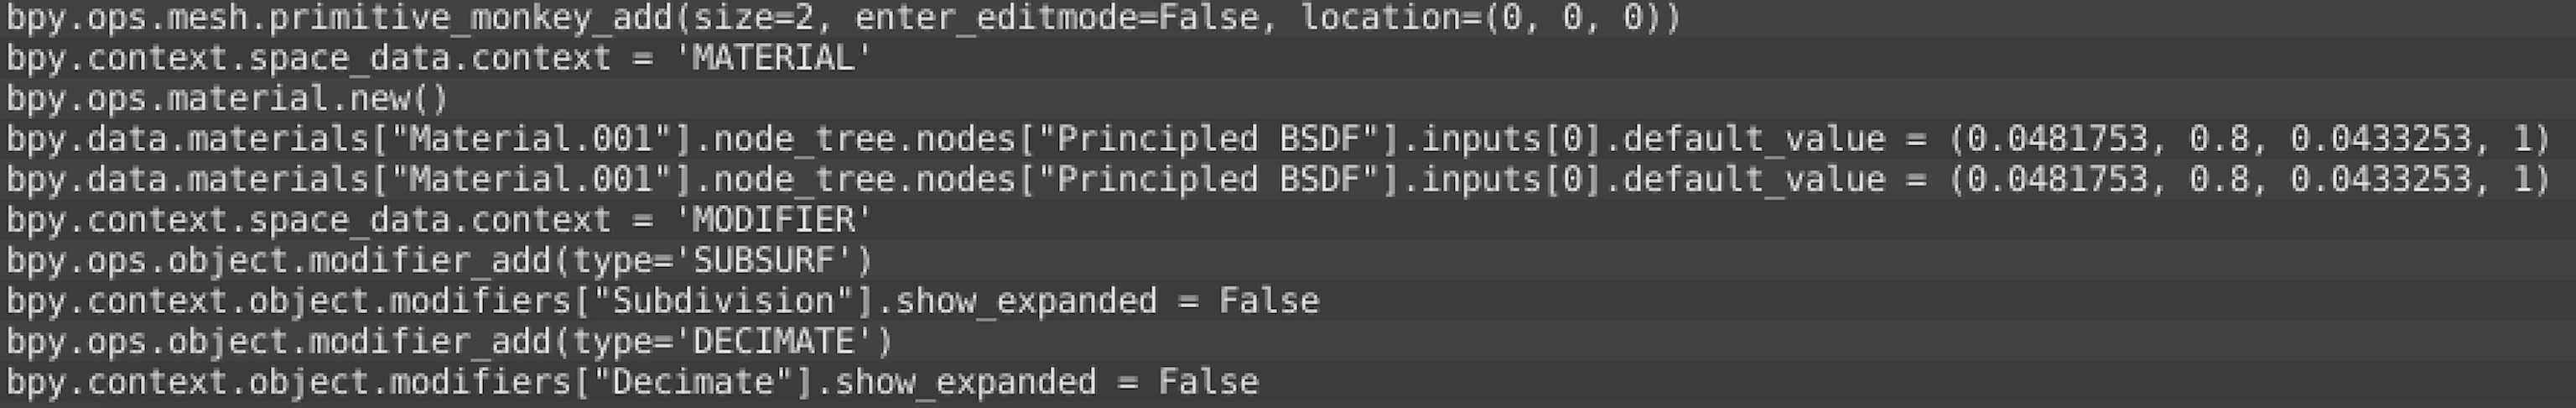
\includegraphics[width=1.1\hsize]{fig/8}
\caption{Przykład prostych operacji w Blenderze, przedstawone w postaci kodu z odwołaniem do BPY. Między innymi znajedzimy tu dodanie nowego materiału, zminę koloru, dodanie modyfikatora Subdivision.\label{RYS.3}}
\source{Opracowanie własne}
\end{figure}
  
\section{NumPy\label{s:dsssl}}
    
    NumPy jest zdecydowanie najpopularniejszą biblioteką wielowymiarową. PyTorch oferuje płynną interoperacyjność z NumPy, co zapewnia integrację z resztą bibliotek naukowych w języku Python, takie jak SciPy, Scikit-learn i Pandas.
    

Tensory PyTorch, w przeciwieństwie z macierzami NumPy, mają zdolność do wykonywania szybkich operacji na graficznych jednostkach przetwarzających (GPU), do dystrybucji operacji na wielu urządzeniach oraz do śledzenia wykresu utworzonych obliczeń. Wszystkie te funkcje są ważne przy wdrażaniu nowoczesnej biblioteki do głębokiego uczenia.


Tensory PyTorch można konwertować na tablice NumPy i odwrotnie. W ten sposób można wykorzystać ogromną liczbę funkcji w szerszym ekosystemie Pythona, który zbudował się wokół typu tablicy NumPy. Brak koniecznoścu kopiowania danych między tensorami, a tablicami NumPy wynika z identycznego systemu zarządzania pamięcią, która współpracuje z protokołem buforującym Pythona. 
Ze względu na jego wszechobecność w ekosystemie nauki danych w Pythonie łatwa zamiana tensora na tablicę NumPy, aby użyć charakterystycznych dla NumPy metod bywa przydatna.

\lstset{caption={Przykład konwersji obrazka w tensor przy użyciu NumPy[13]}}
\begin{lstlisting}
def im_convert(self, tensor):
        image = tensor.to("cpu").clone().detach()
        image = image.numpy().squeeze()
        image = image.transpose(1, 2, 0)
        image = image * np.array((0.5, 0.5, 0.5)) + np.array((0.5, 0.5, 0.5))
        image = image.clip(0, 1)

        return image
\end{lstlisting}

    \section{Torchvision\label{s:dsssl}}
    
    Torchvision składa się z popularnych zestawów danych, architektur modeli i typowych transformacji obrazu. Torchvision udostępnia wiele wytrenowanych zawczasu modeli, które są gotowe do użycia. Między innymi VGG19 używane w tej pracy.
    
\lstset{caption={Przykład pobrania modelu VGG19 przez torchvision, więcej o VGG19 w rozdziale 5.4}}
\begin{lstlisting}
models.vgg19(pretrained=True).features
\end{lstlisting}


\section{Pillow\label{s:dsssl}}
    
   Pillow (\textit{ang. Python Image Library PIL}) dodaje obsługę grafiki np. otwieranie, modyfikowanie, zapisywanie plików graficznych.
   
   \lstset{caption={Przykład importowania obrazka przy pomocy PIL}}
\begin{lstlisting}
image = PIL.Image.open(img_path).convert('RGB')
\end{lstlisting}
   
    
\section{OS\label{s:dsssl}}
        
Biblioteka impermentująca interfejsy systemu operacyjnego. W przypadku tej pracy pozwala wykonać instalację paczek w tle poprzez wykonanie procesu terminalowego w tle. 


\lstset{caption={Przykład funckcji, która wykonuje daną komendę termonalową przy użyciu OS}}
\begin{lstlisting}
# execute terminal command and return output
def exec(cmd):
    stream = os.popen(cmd)
    output = stream.read()
    print(output)
\end{lstlisting}



\chapter{Transfer Stylu }

\section{Ogólne założenia\label{s:dsssl}}

Algorytm Neural-Style opracowany został przez Leona A. Gatysa, Alexandra S. Eckera i Matthiasa Bethge. Neural-Style lub Neural-Transfer pozwala robić zdjęcia i odtwarzać je w nowym stylu artystycznym. Algorytm pobiera dwa obrazy, obraz treści i obraz stylu. Następnie zmienia dane wejściowe, aby przypominały treść obrazu i styl artystyczny obrazu stylu.

Jak zostało wspimniane we wcześniejsczych rodziałach sieci neuronowe zbudowane są z sekwencyjnych warstw, gdzie każda warstwa dokonuje ekstrakcji cech coraz to wyższego poziomu.

Na początku możliwa musi być analiza "stylu" obrazu i odzielenie stylu obrazka od jego zawartości. 
Następnym krokiem jest tranfer tego stylu z jednego obrazka do drugiego.[4]

Na podstawowym poziomie "styl" można interpretować jako kolorystyki (np. dominanata czerwonego) oraz tekstury (fale na całości obrazu).
Styl może też odnosić się do bardziej konkretnych właściwosći np. ruchu pędzla lub techniki malowania. Oczywiście treści i stylu obrazu nie można całkowicie rozdzielić. Podczas syntezy obrazu, który łączy zawartość jednego obrazu ze stylem drugiego, zwykle nie istnieje obraz, który idealnie pasuje do obu ograniczeń jednocześnie. Ponieważ jednak funkcja straty, którą minimalizujemy podczas syntezy obrazu, jest liniową kombinacją funkcji straty odpowiednio dla treści i stylu, możemy płynnie regulować nacisk na każdą rekonstrukcję treści lub stylu.

W przykładzie, w którym algorytm rozpoznawał cyfry, neuronem był pojedynczy piksel ze skalą szarości (\textit{ang. Grayscale}), w przypadku Transferu Stylu mamy dwa obrazki o pełnym  spektrum RGB (red, green, blue), a co za tym idzie neuron będzie bardziej skomplikowany. Podobnie jak w rysunku 2.1. utworzony zostaje model warstw sieci neuronowych. W tym przypadku pierwszą warstwą jest tablica wszystkich pikseli z wartościami RGB z obrazka wejściowego. Ostatnią warstwą  są pixele w tej samej ilości i układzie, ale ze zmienionymi wartościami RGB. 

 \begin{figure}[!tbh]
\centering
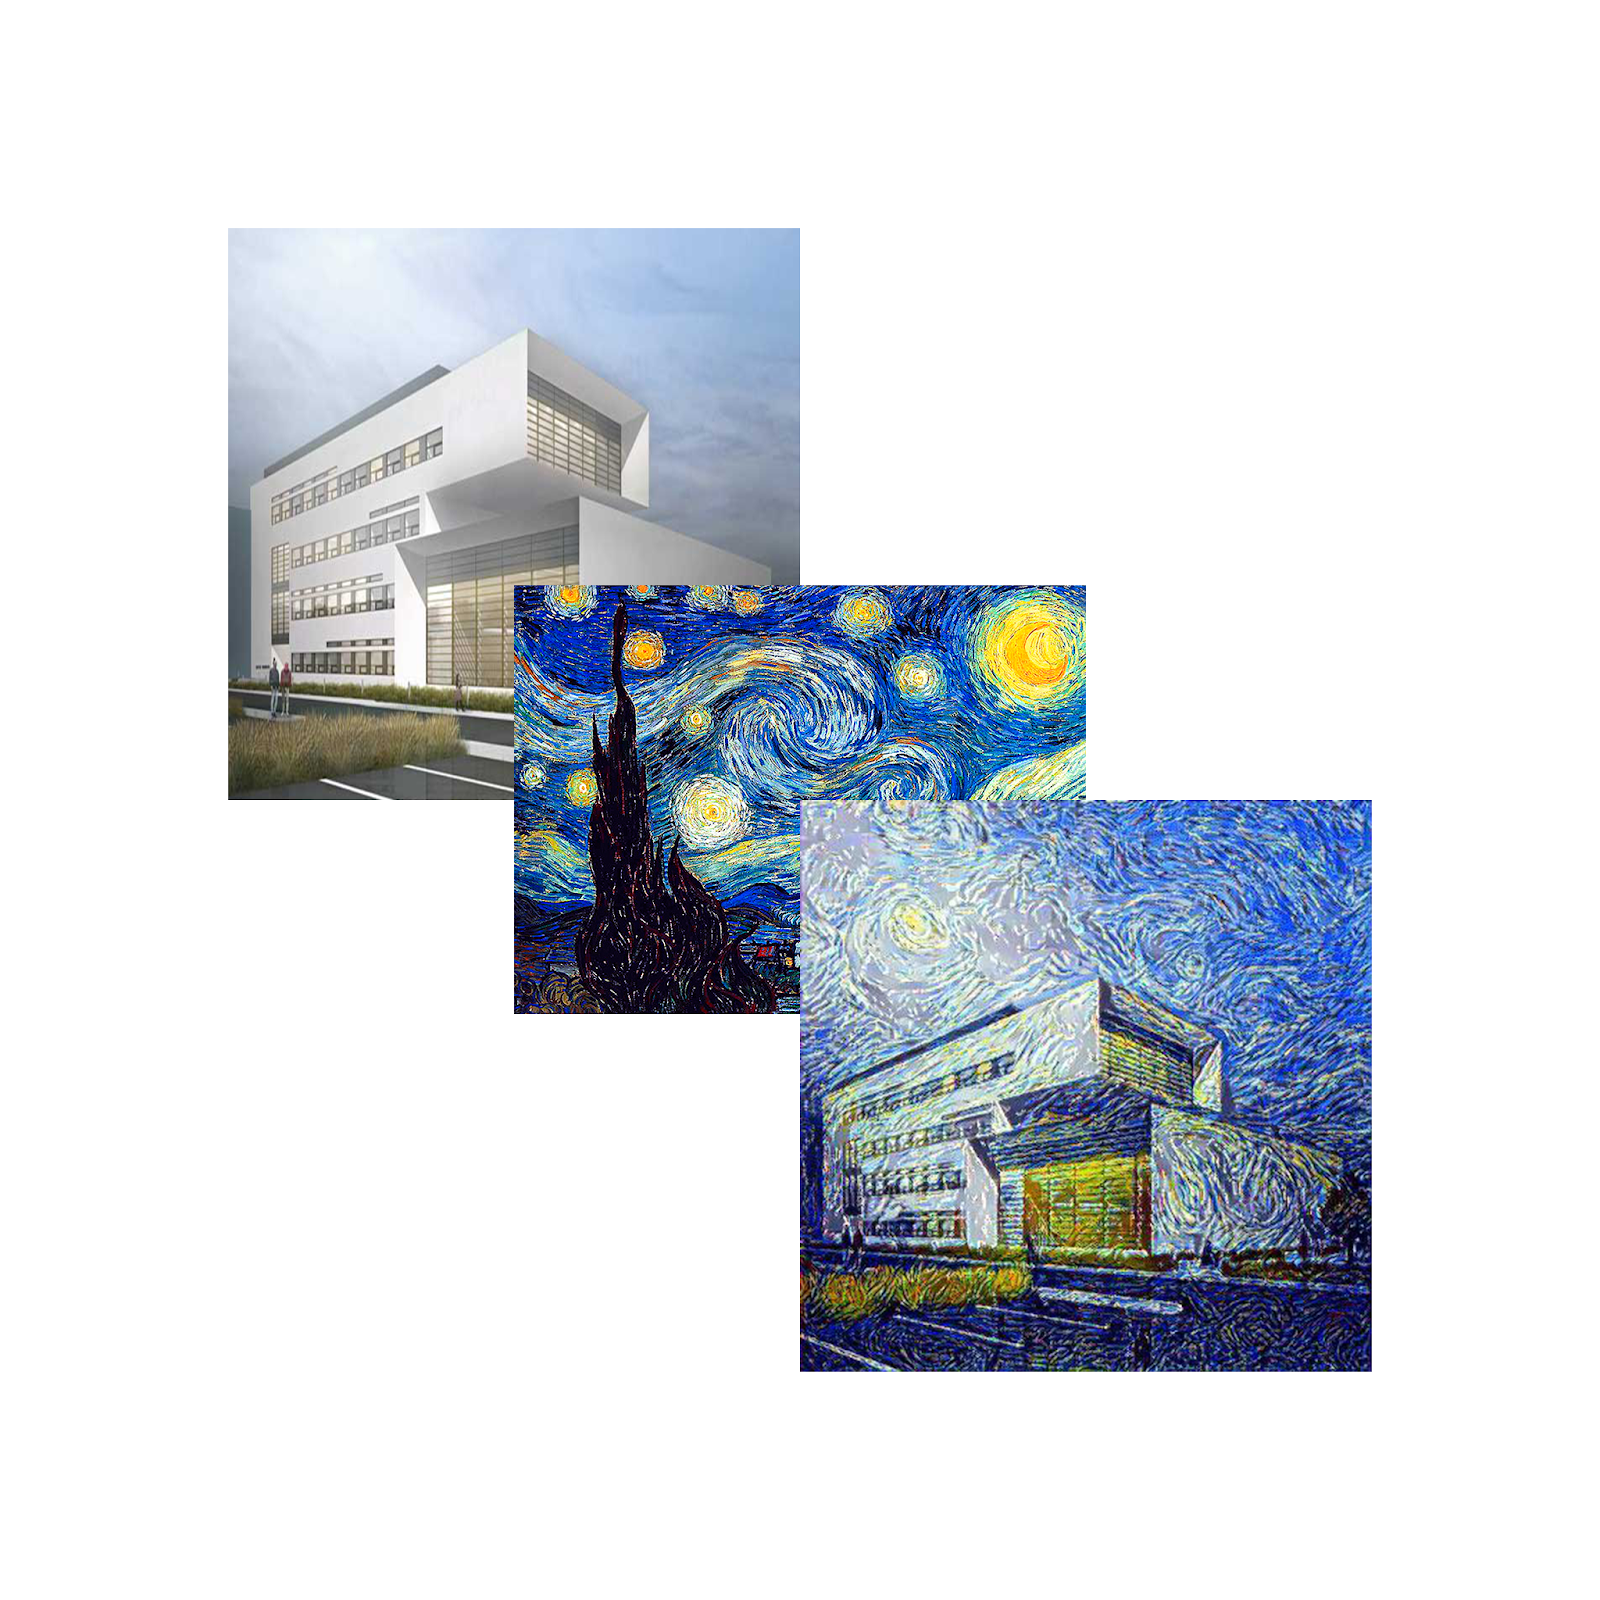
\includegraphics[width=.8\hsize]{fig/6}
\caption{Przykład zastosowania Tranferu Stylu.
Obraz łączący treść zdjęcia ze stylem znanego dzieła sztuki. Obraz został utworzone przez znalezienie obrazu, który jednocześnie pasuje do reprezentacji treści fotografii i stylu kompozycji. Oryginalne zdjęcie przedstawiające wizualizację nowego budynku wydziału Informatyki Uniwersytetu Gdańskiego. Obraz, który zapewnił styl dla odpowiedniego wygenerowanego obrazu to  Gwiaździsta noc Vincenta van Gogha, 1889. Na samym końcu widzimy obraz wyjścia po wykonianiu 2048 iteracji.
\label{RYS.6}}
\source{\textit{https://inf.ug.edu.pl}, Opracowanie własne}
\end{figure}

Oddzielenie treści od stylu w obrazach jest niezwykle trudnym problemem. Jednak ostatni postęp w głębokich konwolucyjnych sieciach neuronowych [4,5,7] stworzył potężne komputerowe systemy interpretacji obrazu, które uczą się wyodrębniać informacje semantyczne na wysokim poziomie z obrazów naturalnych.

Koncepcyjnie jest to algorytm przesyłania tekstur, który ogranicza metodę syntezy tekstur poprzez reprezentacje cech z nowoczesnych konwolucyjnych sieci neuronowych.[4,5,7] Ponieważ model tekstury opiera się również na głębokich reprezentacjach obrazu, metoda transferu stylu ogranicza się do problemu optymalizacji w ramach jednej sieci neuronowej.

Kiedy konwolucyjne sieci neuronowe są szkolone w zakresie rozpoznawania obiektów, rozwijają reprezentację obrazu, która sprawia, że informacje o obiektach stają się coraz bardziej wyraźne wzdłuż hierarchii przetwarzania. Dlatego wzdłuż hierarchii przetwarzania sieci obraz wejściowy przekształca się w reprezentacje, które są coraz bardziej wrażliwe na rzeczywistą treść obrazu, ale stają się względnie niezmienne dla jego dokładnego wyglądu. Zatem wyższe warstwy w sieci wychwytują zawartość wysokiego poziomu w kategoriach obiektów i ich rozmieszczenia w obrazie wejściowym, ale nie ograniczają bardzo dokładnie wartości pikseli w rekonstrukcji. Natomiast rekonstrukcje z niższych warstw po prostu odtwarzają dokładne wartości pikseli oryginalnego obrazu Dlatego też opis funkcji w wyższych warstwach sieci nazywamy reprezentacją treści.


\section{Model\label{s:dsssl}}
Modelem określamy sieć neuronową z dopasowanymi wagami osiągającą wysoką skutecznść np. w przypadku klasyfikacji. Treningiem natomiast określamy proces, w którym wagi modyfikowane są w oparciu o pewną sumę kontrolną lub inny system oceniania.

Aby trenować model, potrzeba:

\begin{itemize}
\item źródła danych treningowych
\item optymalizatora do dostosowania modelu do danych treningowych 
\item pętli  
\item sposobu uzyskania modelu i danych sprzętu, które będą wykonywać obliczenia potrzebne do wyszkolenia modelu

\end{itemize}

Transfer stylu to technika wymagająca bardzo złożonego wytrenowanego modelu. Tutaj przydatne okazują się wytrenowane już modele. VGG19 jest bardzo efektywny przy ekstrakcji cech.

\section{Matryca Gram\label{s:dsssl}}
Aby osięgnąć efektywną jak i efektowną ekstrakcję stylu należy minimalizować różnicę między rozkładami funkcji. Wyciągnięty styl wciąż przechowuje informacje niepotrzebne, takie jak pozycje elementów czy ich strukturę na obrazie. Aby pozbyć się niepotrzebnych informacji trzeba wykonać przetwarzanie wstępne (\textit{ang. Preprocesing}) na macierzy cech, która została wyciągnięta:

\begin{equation}
Gram = V^TV
\end{equation}

gdzie V to dowony wektor będący jedną z cech (\textit{ang. Feature}) w modelu, natomiast T jest transpozycją tego wektora. 
\lstset{caption={Przykład implementacji funkcji, która przetwarza tensor wedle opisanego powyżej wzoru.}}
\begin{lstlisting}
# Gram Matrix
	 def gram(tensor):
	 	 _, d, h, w = tensor.size()
          tensor = tensor.view(d, h * w)
          gram = torch.mm(tensor, tensor.t())
          return gram
\end{lstlisting}


\section{VGG19\label{s:dsssl}}

VGG (\textit{ang. Visual Geometry Group}) to pretrenowany model konwolucyjnej sieci neuronowej. 
Model został wytrenowany na uniwersytecie Oksfordzkim w zakresie rozpoznawania i lokalizacji obiektów na obrazie 2D i jest szczegółowo opisany w oryginalnej pracy [5].

\begin{figure}[!tbh]
\centering
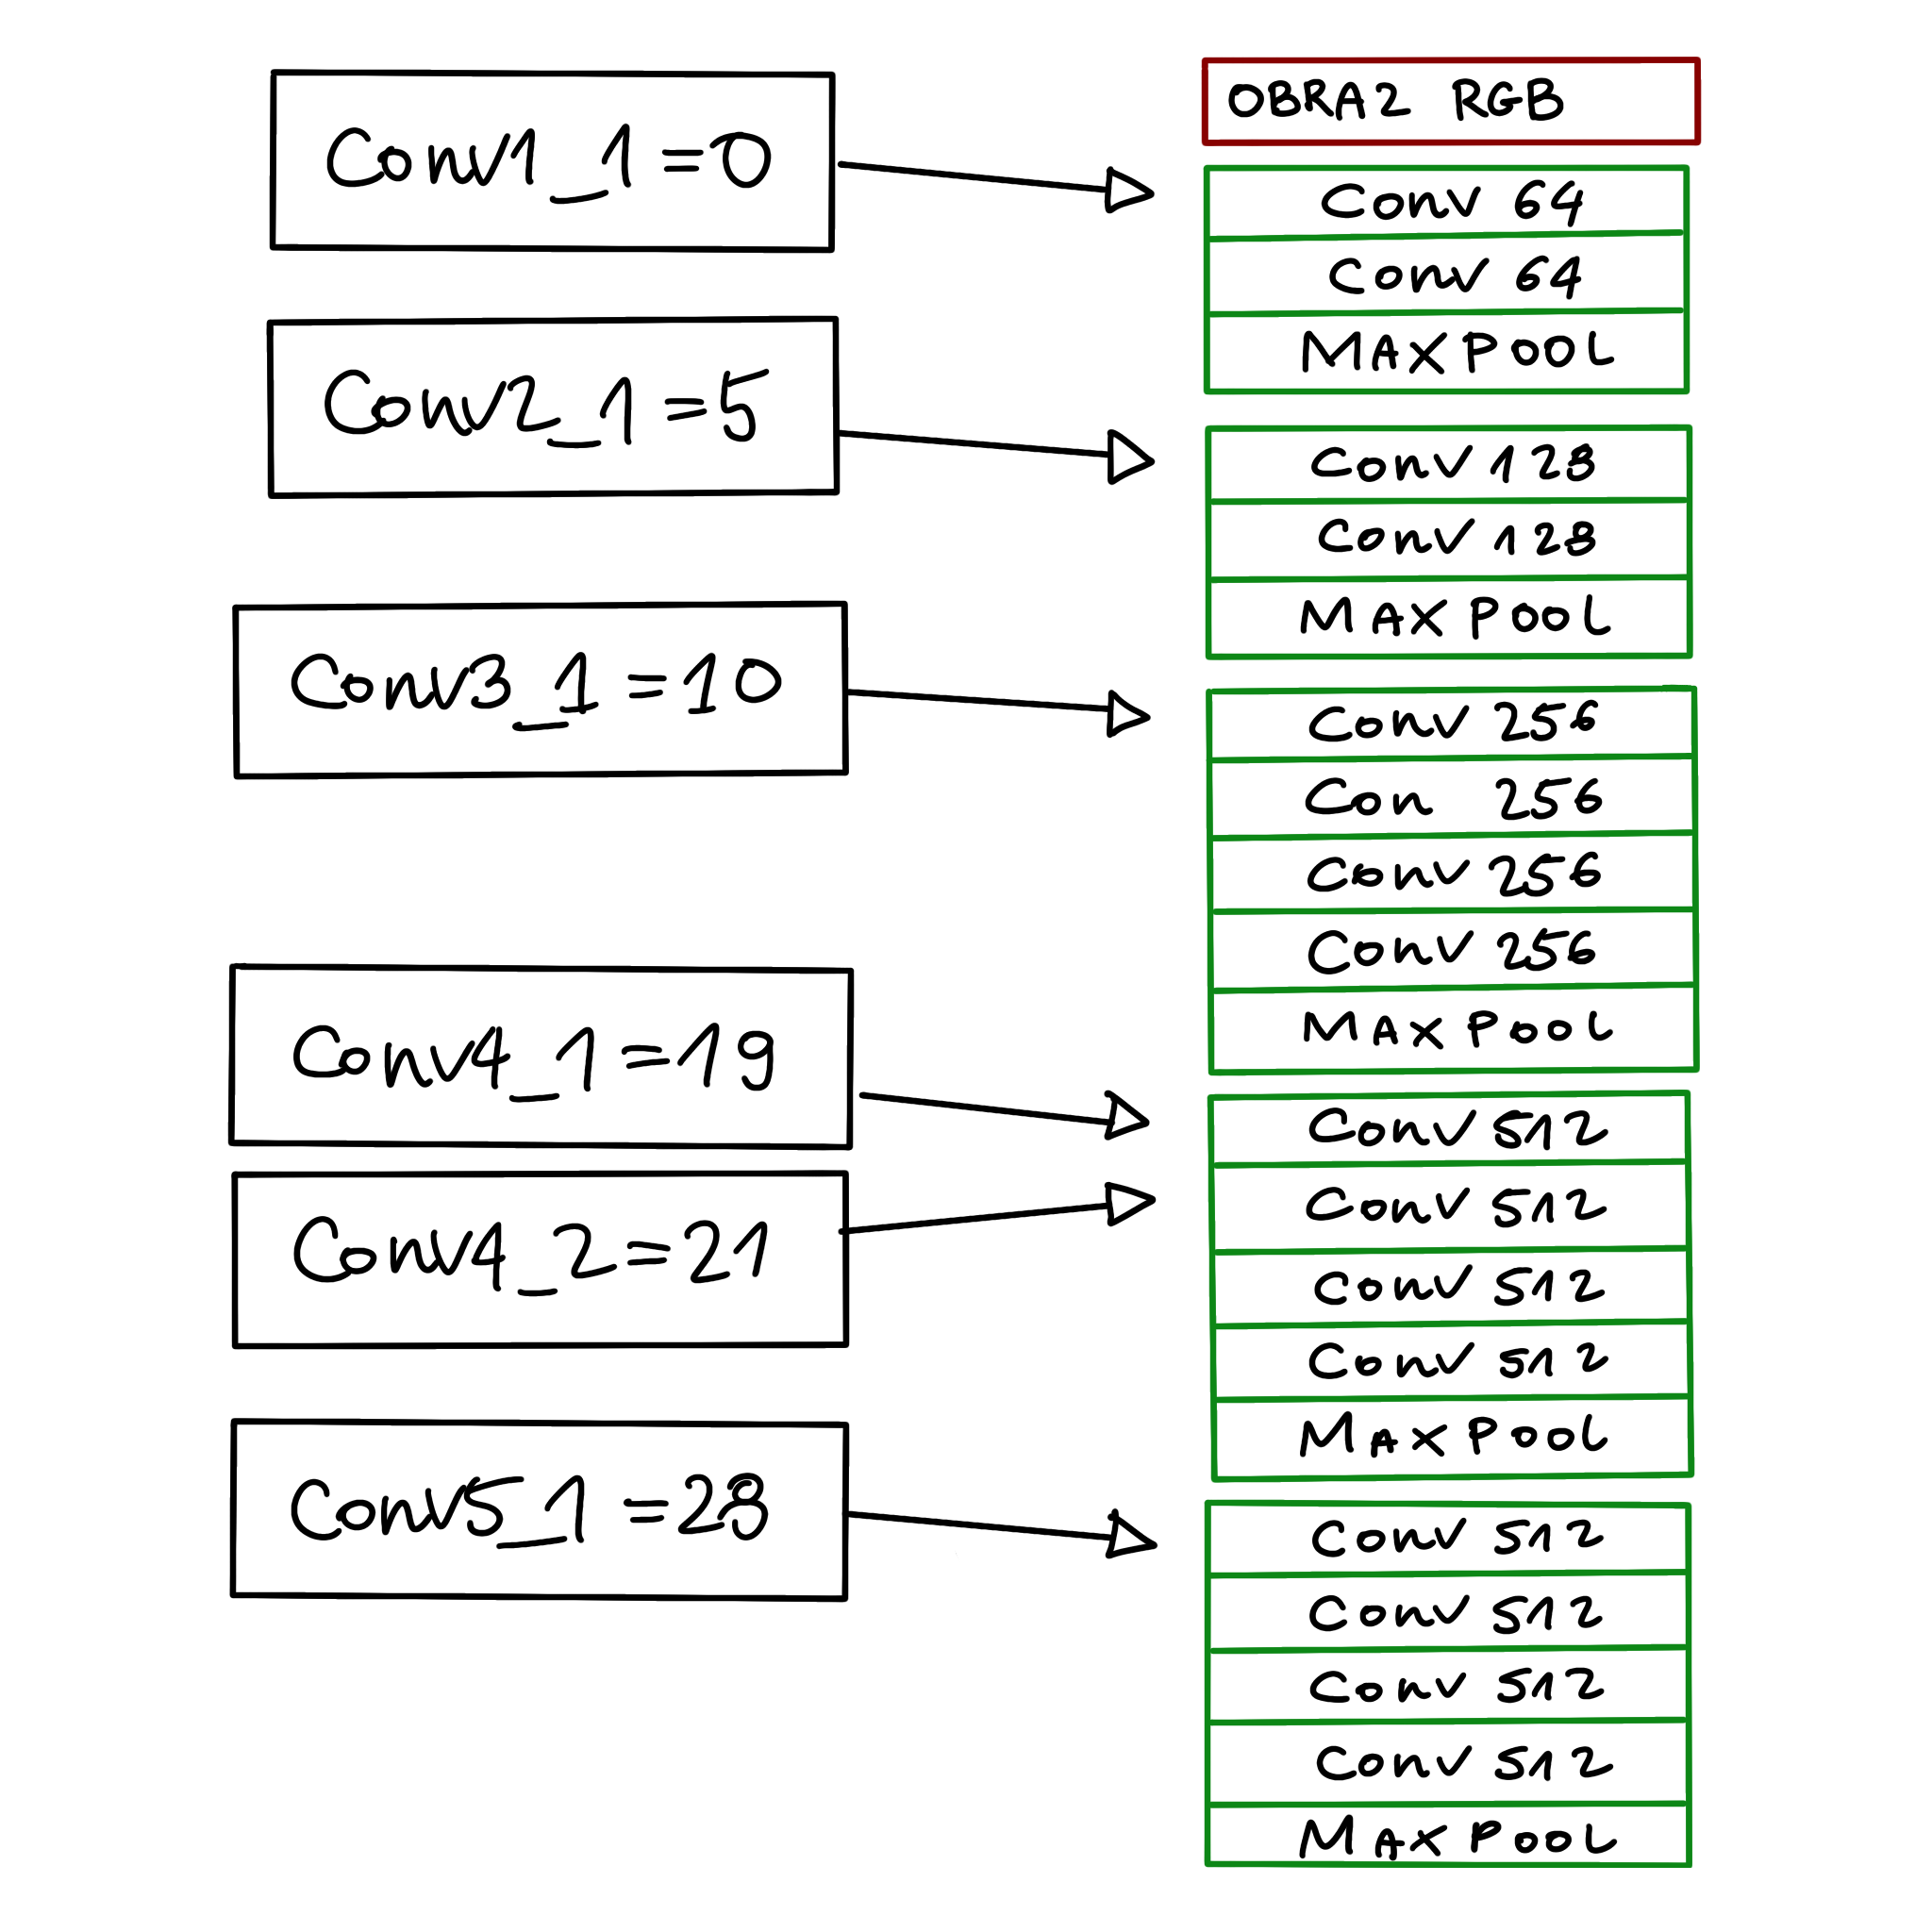
\includegraphics[width=.8\hsize]{fig/7}
\caption{Struktura VGG19\label{RYS.4}}
\source{Opracowanie własne}
\end{figure}


Kluczowa w tym przypaku jest klasyfikacja i wyodrębnianie funkcji.
VGG19 wykorzystuje przestrzeń cech, jaką zapewnia znormalizowana wersja 16 konwolucyjnych, 5 warstw ekstrakcji (\textit{ang. Pooling Layers}) i 19-warstwowej sieci VGG. 

Sieć została znormalizowana poprzez skalowanie wag tak, aby średnia aktywacja każdego filtra konwolucyjnego względem obrazów i pozycji była równa jeden. 

Transfer Stylu nie wymaga używania żadnej z połączonych warstw w pełni. 

Jako, iż VGG19 to wilozadaniowy model, nie wszystkie warstwy będą przydatne przy implementacji Transferu Stylu, potrzebne są tylko te warstwy używane do znajdowania cech. Jest to tylko 6 warstw: warstwy 0, 5, 10, 19, 28 do ekstrakcji stylu oraz warstwa 21 do ekstrakcji kontentu.

\lstset{caption={Przykład implementacji modelu VGG19 [13]}}
\begin{lstlisting}
 # VGG19
model.vgg19(pretrained=True) 
 
def features(image, model):

	layers = {
	'0': 'conv1_1', '5': 'conv2_1', 
	'10': 'conv3_1', '19': 'conv4_1', 
	'21': 'conv4_2', '28': 'conv5_1'
	}

	features = {}

	for name, layer in model._modules.items():
		image = layer(image)
		if name in layers:
			features[layers[name]] = image

	return features
\end{lstlisting}


Reprezentacje treści i stylu w konwolucyjnej sieci neuronowej są rozdzielne w poszczególnych warstwach sieci neuronowej. Oznacza to, że można niezależnie manipulować obiema reprezentacjami, aby wytwarzać nowe, sensownie postrzegalne obrazy. Aby zademonstrować to odkrycie, generujemy obrazy, które mieszają reprezentację treści i stylu z dwóch różnych obrazów źródłowych.

Innym ważnym czynnikiem w procesie syntezy obrazu jest wybór warstw pasujących do treści i reprezentacji stylu. Jak opisano powyżej, reprezentacja stylu jest reprezentacją wielowarstwową, która obejmuje wiele warstw sieci neuronowej. Liczba i położenie tych warstw determinuje lokalną skalę, w której dopasowany jest styl [4]. 
\\
 Najbardziej atrakcyjne wizualnie obrazy są zwykle tworzone przez dopasowanie reprezentacji stylu do wysokich warstw w sieci, dlatego dla wszystkich wyświetlanych obrazów dopasowujemy cechy stylu na warstwach „conv1 1”, „conv2 1”, „conv3 1”, „conv4 1” i „conv5 1” sieci.

\section{Optymalizacja\label{s:dsssl}}

Adam to optymalizator bazujący na metodzie gradientu prostego.

\lstset{caption={Przykład użycia optymalizatora Adam w PyTorch, więcej informacji w rodziale 5.3}}
\begin{lstlisting}

# ustawienie optymalizatora
optimizer = optim.Adam([target], lr=0.003)
      
# reset gradientu
optimizer.zero_grad()
      
# aktualizacja
optimizer.step()

\end{lstlisting}

						
\section{Ograniczenia\label{s:dsssl}}

Prawdopodobnie najbardziej ograniczającym czynnikiem jest rozdzielczość zsyntetyzowanych obrazów. Zarówno problem optymalizacji, jak i liczba jednostek w konwolucyjnej sieci neuronowej rosną wraz z liczbą pikseli, dlatego szybkość procedury syntezy zależy w dużej mierze od rozdzielczości obrazu. Obrazy przedstawione w tej pracy zostały zsyntetyzowane w rozdzielczości około 1024 × 1024 pikseli, a procedura syntezy może zająć nawet godzinę na karcie graficznej NVIDIA GeForce GTX 1060 (M) (Przy użyciu technologii CUDA, o której wiecej w rozdziale 3.6). Podczas gdy ta wydajność obecnie nie sprawdzi się w interaktywnych aplikacjach, prawdopodobne jest, że przyszłe ulepszenia w głębokim uczeniu zwiększą wydajność tej metody.

Inną kwestią jest to, że zsyntetyzowane obrazy narażone są na zakłócenia zwane dalej szumem.  Problem staje się bardziej widoczny, gdy zarówno treść, jak i obrazy w stylu są fotografiami i już na poziomie analizy obraka wejściowego wpływa na wygląd zsyntetyzowanego obrazu. Taki szum jest bardzo charakterystyczny i przypomina filtr. 

Instnieją zaawansowane techniki usuwania sztakich szumów. Takie jak D-Noise Addon dla Blendera od firmy Remington [21] czy NVIDIA OptiX Ray Tracing Engine [22]. Oba rozwiązania korzystają z dobrodziejstw sztuczej ineligencji oraz głębokiego uczenia. Możliwe byłoby skonstruowanie skutecznych technik usuwania szumów w celu późniejszego przetwarzania obrazów po procedurze optymalizacji.
 \\

Oddzielenie treści obrazu od stylu nie jest koniecznie dobrze zdefiniowanym problemem. Wynika to głównie z tego, że nie jest jasne, co dokładnie określa styl obrazu. Mogą to być pociągnięcia pędzlem na obrazie, mapa kolorów, niektóre dominujące formy i kształty, ale także kompozycja sceny i wybór podmiotu obrazu lub jest to połączenie ich wszystkich i wiele więcej. 

\section{Podsumowanie\label{s:dsssl}}

Algorytm Transferu Stylu pozwala (przynajmniej w pewnym stopniu) na oddzielenie treści obrazu od stylu. Jednym z wyjaśnień może być to, że podczas uczenia się rozpoznawania obiektów sieć musi stać się niezmienna dla wszystkich odmian obrazu, które zachowują tożsamość obiektu. Reprezentacje, które uwzględniają zmienność treści obrazu i zmienność jego wyglądu, byłyby niezwykle praktyczne dla tego zadania. W świetle uderzających podobieństw między zoptymalizowanymi pod kątem wydajności sztucznymi sieciami neuronowymi a wizją biologiczną.

\chapter{Zakończenie}
Możliwości jaki stoją przed obrazami generowanymi maszynowo są nieograniczone zarówno do prototypowania i tworzenia "bazy" pomysłów, jak również do odciążania człowieka z zadań które jeszcze kilka lat temu były wykonalne tylko dla najlepszych specjalistów w branży.

W pracy tej zostały przedstawione podstawowe pojęcia związane z sztuczną inteligencją. Następnie omówione zostały sieci neuronowe i widzenie komputerowe jako procesy służące do interpretacji oraz przetwarzania obrazów 2D. 

Aktualnie dostępnych jest szereg narzędzi umożliwiających analizę obrazu, omówione one zostały w rozdziale 4. Dla wcześniej omówionych narzędzi istnieją biblioteki, które pozwalają na wykorzystanie pełnego potencjału uczenia maszynowego i zostały one omówione w rozdziale 5.

Implementacja transferu stylu została szczegółowo omówiona w rozdziale 6. Algorytmu Neural-Style  w środowisku Blender. W tym rozdziale został pokazany cały proces od założeń, przez stworzenie modelu, poprzez szkolenie. Pokazano, że transfer stylu pozwala na analizować zdjęcia i odtwarzać je w nowym stylu artystycznym, ale również ma pewne ograniczenia. 


\chapter{Bibliografia}

\begin{itemize}
\item$[1]\: Alan\:Turing, "Computing\:Machinery\:and \:Intelligence",\\ 
Mind, vol. LIX, no.\:236, Październik 1950$
\item$[2]\: Ian \:Goodfellow \:and \:Yoshua \:Bengio \:and \:Aaron\: Courville,\\ 
"Deep\: Learning\: An\: MIT\: Press\: book",\: https://www.deeplearningbook.org$
\item $[3]\:Vishnu \:Subramanian\: Deep\: Learning\: with \:PyTorch\\ https://arxiv.org/pdf/1508.06576.pdf $ 
\item $[4]\:Leon \:A.\: Gatys,\: Alexander\: S. Ecker,\: Matthias\: Bethge\\ "A \:Neural Algorithm \:of\: Artistic Style" $
\item $[5]\:https://www.cv-foundation.org/openaccess/content\_cvp\r_2016/papers/\\\:Gatys\_Image\_Style\_Transfer\_CVPR\_2016\_paper.pdf$
\item $[6] \:Lemaréchal, C. (2012). "Cauchy\:and \:the \:Gradient \:Method" (PDF).\\ Doc\: Math\: Extra:\: 251–254.$
\item $[7]\:https://papers.nips.cc/paper/5633-texture-syanthesis-using-convolutional-neural-networks.pdf$
\item$[8]\:K. \:Simonyan\: and \:A.\: Zisserman. Very\: Deep\: Convolutional\\ \:Networks\: for\: Large Scale\: Image\: Recognition.\\ arXiv:1409.1556 [cs], Sept. 2014. arXiv: 1409.1556.$
\item $[9]\:Grokking Deep Learning, by Andrew W. Trask$
\item $[10]\:Deep Learning with PyTorch by Eli Stevens and Luca Antiga$
\item $[12]\:https://pytorch.org/tutorials/advanced/neural_style_tutorial.html$
\item $[13]\:https://github.com/rrmina/neural-style-pytorch$
\item $[14]\:https://polycount.com/discussion/205872/creating-images-with-python-in-blender$
\item $[15]\:https://cloud.blender.org/p/scripting-for-artists/5993ed908119170ebb57164b$
\item $[16]\:https://www.3blue1brown.com$
\item $[17]\:https://www.manning.com/books/grokking-deep-learning$
\item $[18]\:https://www.deeplearningbook.org$
\item $[19]\:Deep Learning, by Ian Goodfellow, Yoshua Bengio, and Aaron Courville.$
\item $[20]\:https://pl.wikipedia.org/wiki/Sztuczna_inteligencja$
\item $[21]\:https://remington.pro/software/blender/d-noise/$
\item $[22]\:https://developer.nvidia.com/optix$

\end{itemize}


% załączniki (opcjonalnie):
\appendix
\chapter{Tytuł załącznika jeden}

Treść załącznika jeden.

\chapter{Tytuł załącznika dwa}

Treść załącznika dwa.

% literatura (obowiązkowo):
\bibliographystyle{unsrt}
\bibliography{xml}


\oswiadczenie

\end{document}
